

\section{MPM} \label{Sec:MPM}

\subsection{Introduction}

The material point method (MPM) was described by Sulsky et al.~\cite{sulskycmame,sulskycpc} as
an extension to the FLIP (Fluid-Implicit Particle) method of
Brackbill~\cite{brackbill-ruppel86}, which itself is an
extension of the particle-in-cell (PIC) method of
Harlow~\cite{harlow1963}.  Interestingly, the name ``material point method"
first appeared in the literature two years later in a description of
an axisymmetric form of the method~\cite{sulsky_axisym_1996}.  In both
FLIP and MPM, the basic idea is the same: objects are discretized into
particles, or material points, each of which contains all state data for the
small region of material that it represents.  This includes the position, mass, volume,
velocity, stress and state of deformation of that material.  MPM differs from
other so called ``mesh-free" particle methods in that, while each object
is primarily represented by a collection of particles, a computational mesh
is also an important part of the calculation.  Particles do not interact
with each other directly, rather the particle information is accumulated
to the grid, where the equations of motion are integrated forward in time.
This time advanced solution is then used to update the particle state.

The method usually uses a regular structured grid as a computational mesh.
While this grid, in principle, deforms as the material that it is representing
deforms, at the end of each timestep, it is reset to its original undeformed
position, in effect providing a new computational grid for each timestep.
The use of a regular structured grid for each time step has a number of
computational advantages.  Computation of spatial gradients is simplified.
Mesh entanglement, which can plague fully Lagrangian techniques, such as
the Finite Element Method (FEM), is avoided.  MPM has also been successful
in solving problems involving contact between colliding objects, having an
advantage over FEM in that the use of the regular grid eliminates the
need for doing costly searches for contact surfaces\cite{bard}.

In addition to the advantages that MPM brings, as with any numerical technique, it has its own set of shortcomings.  It is computationally more
expensive than a comparable FEM code.  Accuracy for MPM is typically lower
than FEM, and errors associated with particles moving around the computational
grid can introduce non-physical oscillations into the solution.  Finally,
numerical difficulties can still arise in simulations involving large
deformation that will prematurely terminate the simulation.  The severity of
all of these issues (except for the expense) has been significantly reduced
with the introduction of the Generalized Interpolation Material Point Method,
or GIMP\cite{bardgimp}.  The basic concepts associated with GIMP will be
described below.  Throughout this document, MPM (which
ends up being a special case of GIMP) will frequently be referred to
interchangably with GIMP.

In addition, MPM can be incorporated with a multi-material CFD algorithm
as the structural component in a fluid-structure interaction formulation.
This capability was first demonstrated in the CFDLIB codes from
Los Alamos by Bryan Kashiwa and co-workers\cite{kashiwa2000}.  There, as
in the Uintah-MPMICE component,
MPM serves as the Lagrangian description of the solid
material in a multimaterial CFD code.  Certain elements of the
solution procedure are based in the Eulerian CFD algorithm, including
intermaterial heat and momentum transfer as well as satisfaction
of a multimaterial equation of state.  The use of a Lagrangian method
such as MPM to advance the solution of the solid material eliminates
the diffusion typically associated with Eulerian methods.  The Uintah-MPM
component will be described in later chapter of this manual.

Subsequent sections of this chapter will first give a relatively brief
description of the MPM and GIMP algorithms.  This will, of course, be
focused mainly on describing the capabilities of the Uintah-MPM component.
This is followed by a section that attempts to relate the information in
Section~\ref{Sec:AlgDesc} to the implementation in Uintah.
Following that is a description of the information that goes into an input
file.  Finally, a number of examples are provided, along with representative
results.

\subsection{Algorithm Description} \label{Sec:AlgDesc}

Time and space prohibit an exhaustive description of the theoretical
underpinnings of the Material Point Method.   Here we will concentrate
on the discrete equations that result from applying a weak form analysis
to the governing equations.  The interested reader should
consult \cite{sulskycmame,sulskycpc} for the development of these discrete
equations in MPM, and \cite{bardgimp} for the development of the equations
for the GIMP method.  These end up being very similar, the differences in
how the two developments affect implementation will be described in
Section~\ref{gimp_mpm}.

In solving a structural mechanics problem with MPM, one begins by discretizing
the object of interest into a suitable number of particles, or ``material
points".  ({\bf Aside:}  What constitutes a suitable number is something of an open
question, but it is typically advisable to use at least two particles in each
computational cell in each direction, i.e. 4 particles per cell (PPC) in 2-D,
8 PPC in 3-D. In choosing the resolution of the computational grid, similar
considerations apply as for any computational method (trade-off between
time to solution and accuracy, use of resolution studies to ensure convergence
in results, etc.).)  Each of these particles will carry, minimally, the
following variables:
\begin{itemize}

\item position - $\bfx_p$
\item mass - $m_p$
\item volume - $v_p$
\item velocity - $\bfv_p$
\item stress - $\sig_p$ 
\item deformation gradient - $\bfF_p$

\end{itemize}

The description that follows is a recipe for advancing each of these
variables from the current (discrete) time $n$ to the subsequent
time $n+1$.  Note that particle mass, $m_p$, typically remains constant
throughout a simulation unless solid phase reaction models are utilized,
a feature that is not present in Uintah-MPM.  (Such models are available
in MPMICE, see Section \ref{Sec:MPMICE}.)  It is also important to point
out that the algorithm for advancing the timestep is based on the so-called
Update Stress Last (USL) algorithm.  The superiority of this approach over
the Update Stress First (USF) approach was clearly demonstrated by Wallstedt
and Guilkey \cite{WallstedtJCP}.  USF was the formulation used in Uintah
until mid-2008.

The discrete momentum equation that results from the weak form is given as:
\begin{eqnarray}
        \bfm \bfa &=& \bfF^{\rm{ext}} - \bfF^{\rm{int}}  \label{newton2}
\end{eqnarray}
where $\bfm$ is the mass matrix, $\bfa$ is the acceleration vector,
$\bfF^{\rm{ext}}$ is the external force vector (sum of the body forces and
tractions), and $\bfF^{\rm{int}}$ is the internal force vector resulting from
the divergence of the material stresses.  The construction of each of these
quantities, which are based at the nodes of the computational grid,
will be described below.

The solution begins by accumulating the particle state on the
nodes of the computational grid, to form the mass matrix $\bfm$ and to find
the nodal external forces $\bfF^{\rm{ext}}$, and velocities,
$\bfv$.  In practice, a lumped mass matrix is used to avoid the need to
invert a system of equations to solve Eq. \ref{newton2} for acceleration.
These quantities are calculated at individual nodes by the following equations,
where the $\sum\limits_{p}$ represents a summation over all particles:
\begin{eqnarray}
m_i = \sum_{p} S_{ip} m_p,  \;\;\;\;\;\; 
\bfv_i = \frac{\sum\limits_{p} S_{ip} m_p \bfv_p}{m_i},  \;\;\;\;\;\;
\bfF^{\rm{ext}}_i &=& \sum_{p} S_{ip} \bfF^{\rm{ext}}_p
\label{accumulate}
\end{eqnarray}
and $i$ refers to individual nodes of the grid.  $m_p$ is the particle
mass, $\bfv_p$ is the particle velocity, and $\bfF^{\rm{ext}}_p$ is the
external force on the particle.  The external forces that start on the
particles typically the result of tractions, the application of which will
be discussed in Section \ref{PhysicalBCs}.
$S_{ip}$ is the shape function of the $ith$ node evaluated at $\bfx_p$.
The functional form of the shape functions differs between MPM and GIMP.
This difference is discussed in Section \ref{gimp_mpm}.

Following the operations in Eq.~\ref{accumulate}, $\bfF^{\rm{int}}$
is still required in order to solve for acceleration at the nodes.
This is computed at the nodes as a volume integral of the divergence
of the stress on the particles, specifically:

\begin{eqnarray}
\bfF^{\rm{int}}_i &=& \sum_{p} \bfG_{ip} \sig_p v_p,
\label{computeIntForce}  
\end{eqnarray}
where $\bfG_{ip}$ is the gradient of the shape function of the $ith$ node
evaluated at $\bfx_p$, and $\sig_p$ and $v_p$ are the time $n$ values of
particle stress and volume respectively.  

Equation \ref{newton2} can then be solved for $\bfa$.
\begin{eqnarray}
\bfa_i &=& \frac{\bfF_i^{\rm{ext}} - \bfF_i^{\rm{int}}}{m_i}
\label{MPM:acceleration}
\end{eqnarray}
An explicit forward Euler method is used for the time integration:
\begin{eqnarray}
\bfv_i^L= \bfv_i + \bfa_i \Delta{t}
\label{MPM:euler}
\end{eqnarray}

The time advanced grid velocity, $\bfv^L$ is used to compute a velocity
gradient at each particle according to:

\begin{equation}
\nabla \bfv_p = \sum_i \bfG_{ip} \bfv^L_i
\label{velgrad}
\end{equation}
This velocity gradient is used to update the particle's deformation gradient,
volume and stress.  First, an incremental deformation gradient is computed
using the velocity gradient:

\begin{equation}
\bfd \bfF_p^{n+1} = (\bfI+\nabla \bfv_p \Delta{t})
\label{Finc}
\end{equation}
Particle volume and deformation gradient are updated by:

\begin{eqnarray}
v_p^{n+1} = \rm{Det}(\bfd\bfF_p^{n+1})v_p^n,  \;\;\;\;\;\;\;\;\;
\bfF_p^{n+1}=\bfd\bfF_p^{n+1} \bfF_{p}^{n}
\label{p_vol}
\end{eqnarray}
Finally, the velocity gradient, and/or the deformation gradient are
provided to a constitutive model, which outputs a time advanced stress
at the particles.  Specifics of this operation will be further discussed
in Section~\ref{ConstitutiveModels}

At this point in the timestep, the particle position and velocity are explicitly
updated by:
\begin{eqnarray}
\bfv_p (t + \Delta{t})  &=& \bfv_p (t)  + \sum_{i} S_{ip} \bfa_i  \Delta{t} 
\label{MPM:updateVp}
\end{eqnarray}
\begin{eqnarray}
\bfx_p (t + \Delta{t})  &=& \bfx_p (t)  + \sum_{i} S_{ip} \bfv^L_i  \Delta{t}
\label{MPM:updateXp}
\end{eqnarray}
This completes one timestep, in that the update of all six of the variables
enumerated above (with the exception of mass, which is assumed to remain
constant) has been accomplished.  Conceptually, one can imagine that, since an
acceleration and velocity were computed at the grid, and an interval of time
has passed, the grid nodes also experienced a displacement.  This 
displacement also moved the particles in an isoparametric fashion.  In
practice, particle motion is accomplished by Equation~\ref{MPM:updateXp},
and the grid never deforms.  So, while the MPM literature will often refer
to resetting the grid to its original configuration, in fact, this 
isn't necessary as the grid nodes never leave that configuration.  Regardless,
at this point, one is ready to advance to the next timestep.

The algorithm described above is the core of the Uintah-MPM implementation.
However, it neglects a number of important considerations.  The first is
kinematic boundary conditions on the grid for velocity and acceleration.
The manner in which these are handled will be described in
Section~\ref{Sec:UintahImp}.  Next, is the use of advanced contact
algorithms.  By default, MPM enforces no-slip, no-interpenetration contact.
This feature is extremely useful, but it also means that two bodies initially
in ``contact" (meaning that they both contain particles whose data are
accumulated to common nodes) behave as if they are a single body.  To enable
multi-field simulations with frictional contact, or to impose displacement
based boundary conditions, e.g. a rigid piston, additional steps must be
taken.  These steps implement contact formulations such as that described
by Bardenhagen, et al.\cite{bard_contact}.  The {\it use} of the contact
algorithms is described in Section~\ref{Contact}, but the reader will be
referred to the relevant literature for their development.  Lastly, heat
conduction is also available in the explicit MPM code, although it may be
neglected via a run time option in the input file.  Explicit MPM is typically
used for high rate simulations in which heat conduction is negligible.

\subsection{Shape functions for MPM and GIMP} \label{gimp_mpm}

In both MPM and GIMP, the basic idea is the same: objects are discretized into
particles, or material points, each of which contains all state data for the
small region of material that it represents.  In MPM, these particles are spatially
Dirac delta functions, meaning that the material that each represents is
assumed to exist at a single point in space, namely the position of the
particle.  Interactions between the particles and the grid take place
using weighting functions, also known as shape functions or interpolation
functions.  These are typically, but not necessarily, linear, bilinear or
trilinear in one, two and three dimensions, respectively.

More recently, Bardenhagen and Kober~\cite{bardgimp} generalized the
development that gives rise to MPM, and suggested that MPM
may be thought of as a subset of their ``Generalized Interpolation
Material Point" (GIMP) method.  In the family of GIMP methods
one chooses a characteristic function $\chi_p$ to represent
the particles and a shape function $S_i$ as a basis of support on the
computational nodes.  An effective shape function $\bar{S}_{ip}$  is found
by the convolution of the $\chi_p$ and $S_i$ which is written as:
\begin{equation}
\bar{S}_{ip}(\bfx_p) = \frac{1}{V_p}  \int_{\Omega_p \cap \Omega} \chi_p(\bfx - \bfx_p) S_i(\bfx)\,\mathrm{d}\bfx .
\label{effectiveS}
\end{equation}
While the user has significant latitude in choosing
these two functions, in practice, the choice of $S_i$ is usually given
(in one-dimension) as,
\begin{equation}
S_i\left(x\right) = \begin{cases} 1 + {\left(x-x_i\right) / h} & {-h < x-x_i \le 0} \\
                    1 - {\left(x-x_i\right) / h} & {0  < x-x_i \le h} \\
                    0 & \text{otherwise},
       \end{cases}
\label{linear_shape}
\end{equation}
where $x_i$ is the vertex location, and $h$ is the cell width, 
assumed to be constant in this formulation, 
although this is not a general restriction on the method.
Multi-dimensional versions are constructed by forming tensor products of the
one-dimensional version in the orthogonal directions.  

When the choice of characteristic function is the Dirac delta,
\begin{equation}
\chi_p(\bfx) = \delta(\bfx-\bfx_p)V_p , \label{MPM_char}
\end{equation}
where $\bfx_p$ is the particle position, and $V_p$ is the particle volume,
then traditional MPM is recovered.  In that case, the effective shape function
is still that given by Equation~\ref{linear_shape}.  Its gradient is given by:

\begin{equation}
G_i\left(x\right) = \begin{cases} {1 / h} & {-h < x-x_i \le 0} \\
                    {-1 / h} & {0  < x-x_i \le h} \\
                    0 & \text{otherwise},
       \end{cases}
\label{linear_shape_grad}
\end{equation}

Plots of Equations~\ref{linear_shape} and~\ref{linear_shape_grad} are shown
below.  The discontinuity in the gradient gives rise to poor accuracy and
stability properties.

\begin{figure}
  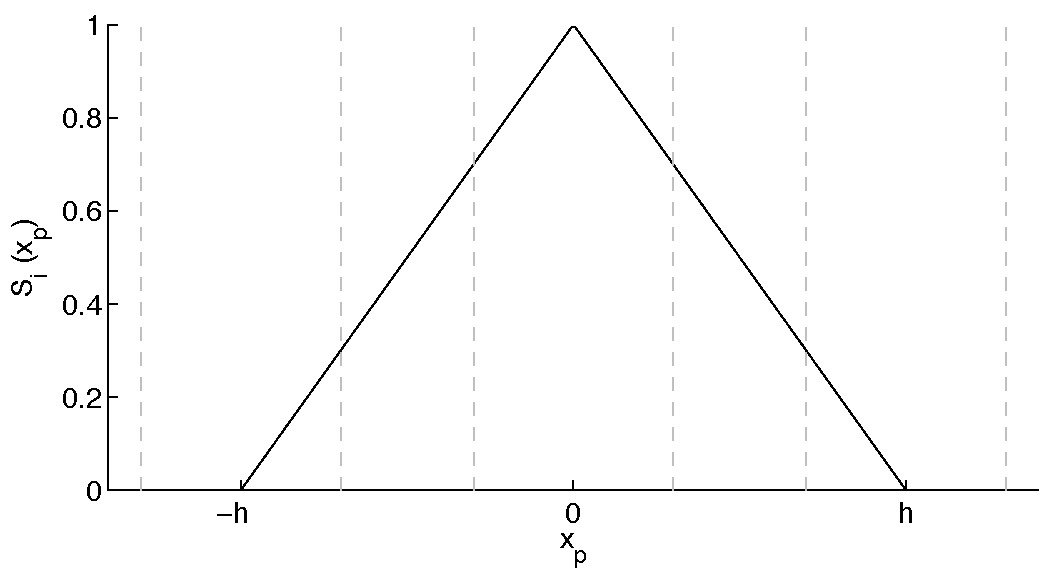
\includegraphics[scale=.85]{mpm_basis.pdf}
  \caption{Effective shape function when using traditional MPM.}
  \label{Fig:MPMShape}
\end{figure}

\begin{figure}
  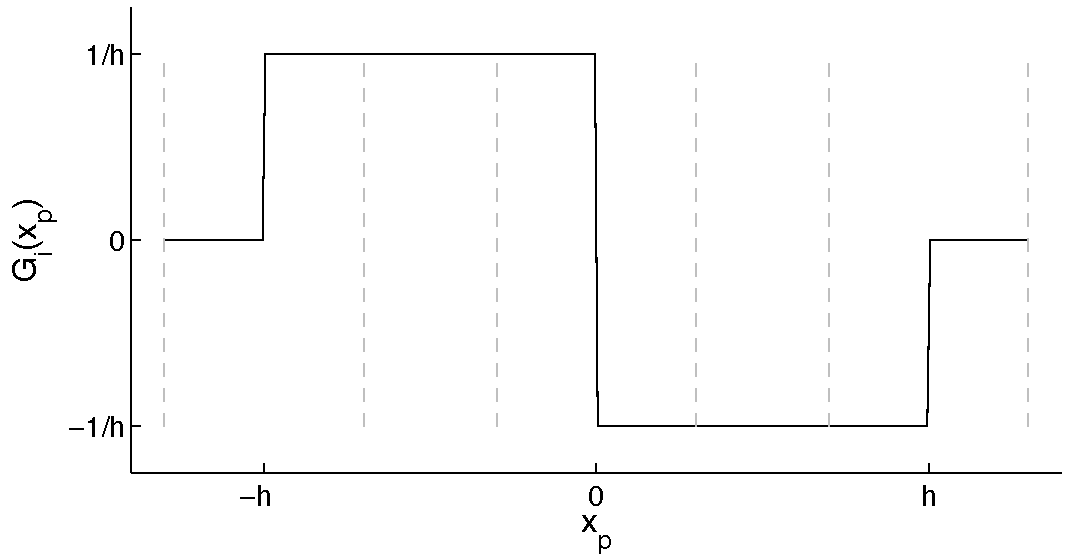
\includegraphics[scale=.85]{mpm_grad.pdf}
  \caption{Gradient of the effective shape function when using traditional MPM.}
  \label{Fig:MPMShapeGrad}
\end{figure}

Typically, when an analyst indicates that
they are ``using GIMP" this implies use of the linear grid basis function
given in Eq.~\ref{linear_shape} and a ``top-hat" characteristic function,
given by (in one-dimension),
\begin{equation}
\chi_p(x) = H(x-(x_p-l_p))-H(x-(x_p+l_p)) , \label{GIMP_char}
\end{equation}
where $H(x)$ is the Heaviside function
($H(x)=0$ if $x<0$ and $H(x)=1$ if $x\ge0$) and $l_p$ is the half-length
of the particle.  When the convolution indicated in Eq.~\ref{effectiveS}
is carried out using the expressions in Eqns.~\ref{linear_shape}
 and~\ref{GIMP_char}, a closed form for the effective shape function can be
written as:
\begin{equation}
S_{i}\left(x_p\right) = \begin{cases}
   \frac{\left(h+l_p+\left(x_p-x_i\right)\right)^2}{4hl_p} & {-h -l_p < x_p-x_i \le -h+l_p} \\
   1 + \frac{\left(x_p-x_i\right)}{h} & {-h + l_p < x_p-x_i \le -l_p} \\
   1 - \frac{\left(x_p-x_i\right)^2 + l_p^2}{2hl_p} & {-l_p < x_p-x_i \le l_p} \\
   1 - \frac{\left(x_p-x_i\right)}{h} & {l_p  < x_p-x_i \le h-l_p} \\
   \frac{\left(h+l_p-\left(x_p-x_i\right)\right)^2}{4hl_p} & {h -l_p < x_p-x_i \le h+l_p} \\
   0 & \text{otherwise},
\end{cases}
\label{gimp_shape}
\end{equation}
%
The gradient of which is:
\begin{equation}
G_i(x_p) = \begin{cases}
   \frac{h+l_p+\left(x_p-x_i\right)}{2 h l_p} & {-h -l_p < x_p-x_i \le -h+l_p} \\
   \frac{1}{h} & {-h + l_p < x_p-x_i \le -l_p} \\
   - \frac{\left(x_p-x_i\right)}{h l_p} & {-l_p < x_p-x_i \le l_p} \\
   - \frac{1}{h} & {l_p  < x_p-x_i \le h-l_p} \\
   - \frac{h+l_p-\left(x_p-x_i\right)}{2 h l_p} & {h -l_p < x_p-x_i \le h+l_p} \\
   0 & \text{otherwise},
\end{cases}
\label{gimpGrad}
\end{equation}

Plots of Equations~\ref{gimp_shape} and~\ref{gimpGrad} are shown
below.  The continuous nature of the gradients are largely responsible
for the improved robustness and accuracy of GIMP over MPM.

\begin{figure}
  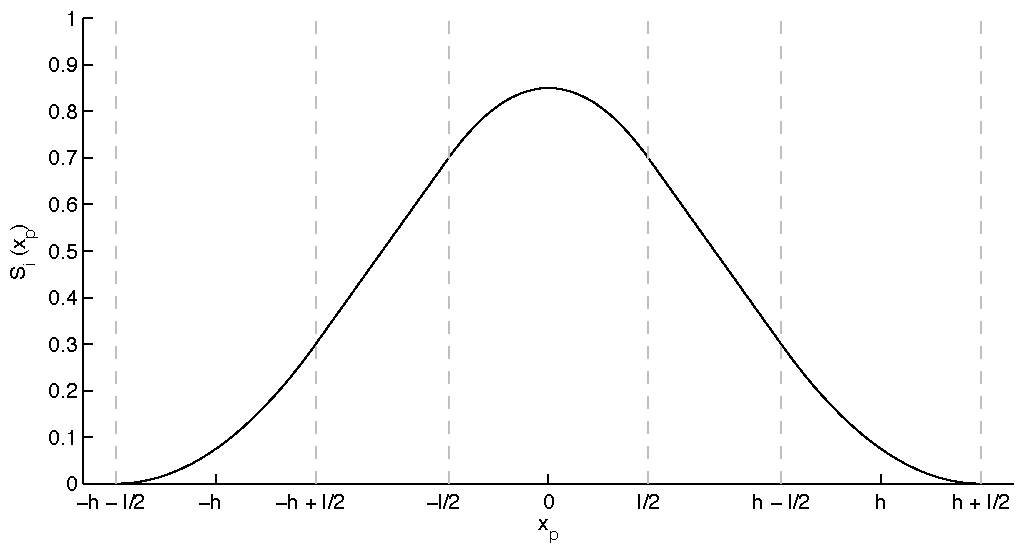
\includegraphics[scale=.85]{gimp_basis.pdf}
  \caption{Effective shape function when using GIMP.}
  \label{Fig:GIMP}
\end{figure}

\begin{figure}
  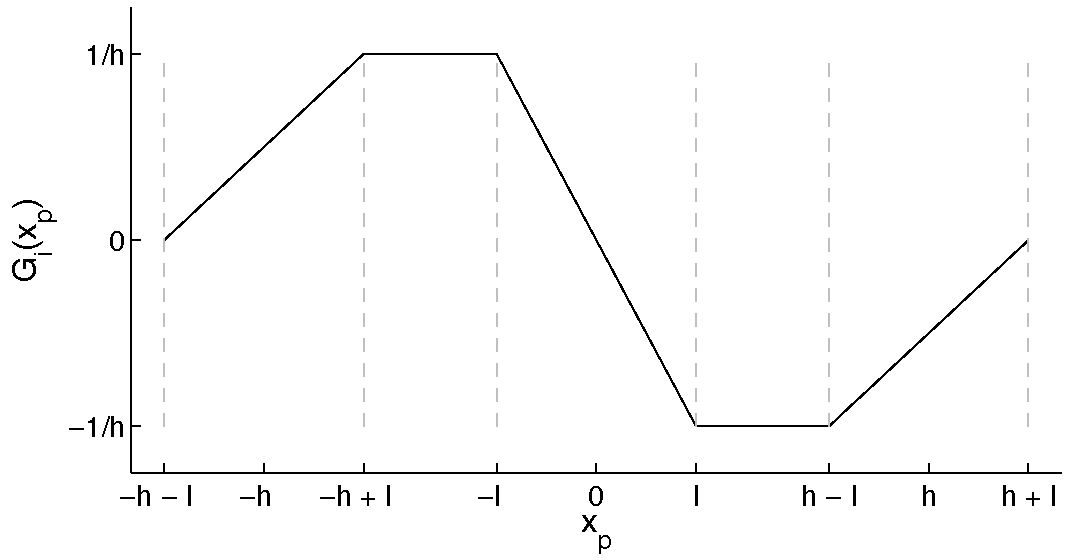
\includegraphics[scale=.85]{gimp_grad.pdf}
  \caption{Gradient of the effective shape function when using GIMP.}
  \label{Fig:GradGIMP}
\end{figure}
%
There is one further consideration in defining the effective shape function,
and that is whether or not the size (length in 1-D) of the particle is kept
fixed (denoted as ``UGIMP" here)
or is allowed to evolve due to material deformations 
(``Finite GIMP" or ``Contiguous GIMP" in (1) and ``cpGIMP" here).
In one-dimensional
simulations, evolution of the particle (half-)length is straightforward,
\begin{equation}
l_p^n = F_p^n l_p^0 ,  \label{particle_length}
\end{equation} 
where $F_p^n$ is the deformation gradient at time $n$.
In multi-dimensional simulations, a similar approach can be used, assuming
an initially rectangular or cuboid particle, to find the current particle
shape.  The difficulty arises in evaluating Eq.~\ref{effectiveS} for
these general shapes.  One approach, apparently effective, has been to create
a cuboid that circumscribes the deformed particle shape~\cite{jinmaCMES2006}.
Alternatively, one can assume that the particle size remains constant (insofar
as it applies to the effective shape function evaluations only).  This is
the approach currently implemented in Uintah.

\subsection{Uintah Implementation} \label{Sec:UintahImp}

Users of Uintah-MPM needn't necessarily bother themselves with the
implementation in code of the algorithm described above.  This section
is intended to serve as a reference for users who find themselves needing
to modify the source code, or those who are simply interested.  Anyone
just wishing to run MPM simulations may skip ahead to
Sections~\ref{Sec:UintahSpecMPM} and~\ref{Sec:ExamplesMPM}.  The goal of
this section is to provide a mapping from the the algorithm described above
to the software that carries it out.  This won't be exhaustive, but will be a
good starting point for the motivated reader.

The source code for the Uintah-MPM implementation can be found in

\begin{Verbatim}[fontsize=\footnotesize]
src/CCA/Components/MPM
\end{Verbatim}
Within that directory are a number of files and subdirectories, these will be
discussed as needed.  For the moment, consider the various files that end in
``{MPM.cc}":
\begin{Verbatim}[fontsize=\footnotesize]
AMRMPM.cc  FractureMPM.cc  ImpMPM.cc  RigidMPM.cc  SerialMPM.cc  ShellMPM.cc
\end{Verbatim}

\tt AMRMPM.cc \normalfont is the nascent beginnings of an AMR implementation of MPM. 
It is far from complete and should be ignored.  \tt FractureMPM.cc \normalfont is an implementation of
the work of Guo and Nairn \cite{GuoNairn}, and while it is viable, it is
undocumented and unsupported.  \tt ShellMPM.cc \normalfont is a treatment of MPM particles
as shell and membrane elements, developed by Biswajit Bannerjee.  It is also
viable, but also undocumented and unsupported.  \tt ImpMPM.cc \normalfont is an implicit
time integration form of MPM based on the work of Guilkey and Weiss
\cite{Guilkey03}.  It is also viable, and future releases of Uintah will include
documentation of its capabilities and uses.  For now, interested readers
should contact Jim Guilkey directly for more information.  \tt RigidMPM.cc \normalfont contains
a very reduced level of functionality, and is used solely in conjunction with
the MPMArches component.

This leaves \tt SerialMPM.cc. \normalfont  This contains, despite its name, the parallel
implementation of the algorithm described above in Section~\ref{Sec:AlgDesc}.
For now, we will skip over the initialization procedures such as:
\begin{Verbatim}[fontsize=\footnotesize]
SerialMPM::problemSetup
SerialMPM::scheduleInitialize
SerialMPM::actuallyInitialize
\end{Verbatim}
and focus mainly on the timestepping algorithm described above.  Reference
will be made back to these functions as needed in
Section~\ref{Sec:UintahSpecMPM}.

Each of the Uintah components contains a function called  \tt scheduleTimeAdvance \normalfont.
The algorithms implemented in these components are broken into a number
of steps.  The implementation of these steps in Uintah take place in ``tasks".
Each task is responsible for performing the calculations needed to accomplish
that step in the algorithm.  Thus, each task requires some data upon which
to operate, and it also creates some data, either as a final result, or as
input to a subsequent task.  Before individual tasks are executed, each is
first ``scheduled".  The scheduling of tasks describes the dataflow and data
dependencies for a given algorithm.  By describing the data dependencies,
both temporally and spatially, each task can be executed in the proper order,
and communication tasks can automatically be generated by the Uintah
infrastructure to achieve parallelism.  Thus, scheduleTimeAdvance calls
a series of functions, each of which schedules the individual tasks.  Let's
begin by looking at the \tt scheduleTimeAdvance \normalfont for \tt SerialMPM, \normalfont pasted below.

\begin{Verbatim}[fontsize=\footnotesize]
void
SerialMPM::scheduleTimeAdvance(const LevelP & level,
                               SchedulerP   & sched)
{
  MALLOC_TRACE_TAG_SCOPE("SerialMPM::scheduleTimeAdvance()");
  if (!flags->doMPMOnLevel(level->getIndex(), level->getGrid()->numLevels()))
    return;

  const PatchSet* patches = level->eachPatch();
  const MaterialSet* matls = d_sharedState->allMPMMaterials();

  scheduleApplyExternalLoads(             sched, patches, matls);
  scheduleInterpolateParticlesToGrid(     sched, patches, matls);
  scheduleExMomInterpolated(              sched, patches, matls);
  scheduleComputeContactArea(             sched, patches, matls);
  scheduleComputeInternalForce(           sched, patches, matls);

  scheduleComputeAndIntegrateAcceleration(sched, patches, matls);
  scheduleExMomIntegrated(                sched, patches, matls);
  scheduleSetGridBoundaryConditions(      sched, patches, matls);
  scheduleSetPrescribedMotion(            sched, patches, matls);
  scheduleComputeStressTensor(            sched, patches, matls);
  if(flags->d_doExplicitHeatConduction){
    scheduleComputeHeatExchange(          sched, patches, matls);
    scheduleComputeInternalHeatRate(      sched, patches, matls);
    scheduleComputeNodalHeatFlux(         sched, patches, matls);
    scheduleSolveHeatEquations(           sched, patches, matls);
    scheduleIntegrateTemperatureRate(     sched, patches, matls);
  }
  scheduleAddNewParticles(                sched, patches, matls);
  scheduleConvertLocalizedParticles(      sched, patches, matls);
  scheduleInterpolateToParticlesAndUpdate(sched, patches, matls);

  if(flags->d_canAddMPMMaterial){
    //  This checks to see if the model on THIS patch says that it's
    //  time to add a new material
    scheduleCheckNeedAddMPMMaterial(         sched, patches, matls);

    //  This one checks to see if the model on ANY patch says that it's
    //  time to add a new material
    scheduleSetNeedAddMaterialFlag(         sched, level,   matls);
  }

  sched->scheduleParticleRelocation(level, lb->pXLabel_preReloc,
                                    d_sharedState->d_particleState_preReloc,
                                    lb->pXLabel,
                                    d_sharedState->d_particleState,
                                    lb->pParticleIDLabel, matls);
  if(d_analysisModule){
    d_analysisModule->scheduleDoAnalysis( sched, level);
  }
}
\end{Verbatim}

The preceding includes scheduling for a number of rarely used features.
For now, let's condense the preceding to the essential tasks:

\begin{Verbatim}[fontsize=\footnotesize]
void
SerialMPM::scheduleTimeAdvance(const LevelP & level,
                               SchedulerP   & sched)
{
  if (!flags->doMPMOnLevel(level->getIndex(), level->getGrid()->numLevels()))
    return;

  const PatchSet* patches = level->eachPatch();
  const MaterialSet* matls = d_sharedState->allMPMMaterials();

  scheduleApplyExternalLoads(             sched, patches, matls);
  scheduleInterpolateParticlesToGrid(     sched, patches, matls);
  scheduleExMomInterpolated(              sched, patches, matls);
  scheduleComputeInternalForce(           sched, patches, matls);

  scheduleComputeAndIntegrateAcceleration(sched, patches, matls);
  scheduleExMomIntegrated(                sched, patches, matls);
  scheduleSetGridBoundaryConditions(      sched, patches, matls);
  scheduleComputeStressTensor(            sched, patches, matls);
  scheduleInterpolateToParticlesAndUpdate(sched, patches, matls);

  sched->scheduleParticleRelocation(level, lb->pXLabel_preReloc,
                                    d_sharedState->d_particleState_preReloc,
                                    lb->pXLabel,
                                    d_sharedState->d_particleState,
                                    lb->pParticleIDLabel, matls);
}
\end{Verbatim}

As described above, each of the ``schedule" functions describes dataflow,
and it also calls the function that actually executes the task.  The naming
convention is illustrated by an example,
\tt scheduleComputeAndIntegrateAcceleration \normalfont calls \tt computeAndIntegrateAcceleration. \normalfont
Let's examine this particular task, which executes
Equations~\ref{MPM:acceleration} and~\ref{MPM:euler}, more carefully.  First,
the scheduling of the task:

\begin{Verbatim}[fontsize=\footnotesize]
void SerialMPM::scheduleComputeAndIntegrateAcceleration(SchedulerP& sched,
                                                       const PatchSet* patches,
                                                       const MaterialSet* matls)
{
  if (!flags->doMPMOnLevel(getLevel(patches)->getIndex(),
                           getLevel(patches)->getGrid()->numLevels()))
    return;

  printSchedule(patches,cout_doing,"MPM::scheduleComputeAndIntegrateAcceleration\t\t\t\t");

  Task* t = scinew Task("MPM::computeAndIntegrateAcceleration",
                        this, &SerialMPM::computeAndIntegrateAcceleration);

  t->requires(Task::OldDW, d_sharedState->get_delt_label() );

  t->requires(Task::NewDW, lb->gMassLabel,          Ghost::None);
  t->requires(Task::NewDW, lb->gInternalForceLabel, Ghost::None);
  t->requires(Task::NewDW, lb->gExternalForceLabel, Ghost::None);
  t->requires(Task::NewDW, lb->gVelocityLabel,      Ghost::None);

  t->computes(lb->gVelocityStarLabel);
  t->computes(lb->gAccelerationLabel);

  sched->addTask(t, patches, matls);
}
\end{Verbatim}

The \tt if \normalfont statement basically directs the schedule to only do this task on the 
finest level (MPM can be used in AMR simulations, but only at the finest
level.)  The \tt printSchedule \normalfont command is in place for debugging purposes,
this type of print statement can be turned on by setting an environmental
variable.  The real business of this task begins with the declaration of the
Task.  In the task declaration, the function associated with that task is
identified.  Subsequent to that is a description of the data dependencies.
Namely, this task \tt requires \normalfont the mass, internal and external forces as well
as velocity on the grid.  No ghost data are required as this task is a 
node by node calculation.  It also requires the timestep size.  Note also
that most of the required data are needed from the \tt NewDW \normalfont where
\tt DW \normalfont refers to
DataWarehouse.  This simply means that these data were calculated by an
earlier task in the current timestep.  The timestep size for this step
was computed in the previous timestep, and thus is required from the \tt OldDW. \normalfont
Finally, this task \tt computes \normalfont the acceleration and time advanced velocity
at each node.

The code to execute this task is as follows:

\begin{Verbatim}[fontsize=\footnotesize]
void SerialMPM::computeAndIntegrateAcceleration(const ProcessorGroup*,
                                                const PatchSubset* patches,
                                                const MaterialSubset*,
                                                DataWarehouse* old_dw,
                                                DataWarehouse* new_dw)
{
  for(int p=0;p<patches->size();p++){
    const Patch* patch = patches->get(p);
    printTask(patches, patch,cout_doing,"Doing computeAndIntegrateAcceleration\t\t\t\t");

    Ghost::GhostType  gnone = Ghost::None;
    Vector gravity = d_sharedState->getGravity();
    for(int m = 0; m < d_sharedState->getNumMPMMatls(); m++){
      MPMMaterial* mpm_matl = d_sharedState->getMPMMaterial( m );
      int dwi = mpm_matl->getDWIndex();

      // Get required variables for this patch
      constNCVariable<Vector> internalforce, externalforce, velocity;
      constNCVariable<double> mass;

      delt_vartype delT;
      old_dw->get(delT, d_sharedState->get_delt_label(), getLevel(patches) );

      new_dw->get(internalforce,lb->gInternalForceLabel, dwi, patch, gnone, 0);
      new_dw->get(externalforce,lb->gExternalForceLabel, dwi, patch, gnone, 0);
      new_dw->get(mass,         lb->gMassLabel,          dwi, patch, gnone, 0);
      new_dw->get(velocity,     lb->gVelocityLabel,      dwi, patch, gnone, 0);

      // Create variables for the results
      NCVariable<Vector> velocity_star,acceleration;
      new_dw->allocateAndPut(velocity_star, lb->gVelocityStarLabel, dwi, patch);
      new_dw->allocateAndPut(acceleration,  lb->gAccelerationLabel, dwi, patch);

      acceleration.initialize(Vector(0.,0.,0.));
      double damp_coef = flags->d_artificialDampCoeff;

      for(NodeIterator iter=patch->getExtraNodeIterator__New();
                        !iter.done();iter++){
        IntVector c = *iter;
        Vector acc(0.,0.,0.);
        if (mass[c] > flags->d_min_mass_for_acceleration){
          acc  = (internalforce[c] + externalforce[c])/mass[c];
          acc -= damp_coef*velocity[c];
        }
        acceleration[c] = acc +  gravity;
        velocity_star[c] = velocity[c] + acceleration[c] * delT;
      }
    }    // matls
  }
}
\end{Verbatim}

This task contains three nested for loops.  First, is a loop over all of the
``patches" that the processor executing this task is responsible for.  Next
is a loop over all materials (imagine a simulation involving the interaction
between, say, tungsten and copper).  Within this loop, the required data
are retrieved from the \tt new\_dw \normalfont (New DataWarehouse) and space for the data
to be created is allocated.  The final loop is over all of the nodes on
the current patch, and the calculations described by
Equations~\ref{MPM:acceleration} and~\ref{MPM:euler} are carried out.  (This
also includes a linear damping term not described above.)

Let's consider each task in turn.  The remaining tasks will be described
in much less detail, but the preceding dissection of a fairly simple task,
along with a description of what the remaining tasks are intended to 
accomplish, should allow interested individuals to follow the remainder
of the Uintah-MPM implementation.

\begin{enumerate}
\item {\tt scheduleApplyExternalLoads \normalfont} This task is mainly responsible for
applying traction boundary conditions described in the input file.  This is
done by assigning external force vectors to the particles.  If the user
wishes to apply a load that is not possible to acheive via the input file
options, it is straightforward to modify the code here to do ``one-off" tests.

\item {\tt scheduleInterpolateParticlesToGrid \normalfont}   The name of this task was
poorly chosen, but has persisted.  This task carries out the operations given
in Equation~\ref{accumulate}.  It also sets boundary conditions on some of
the variables, such as the grid temperature, and grid velocity 
(in the case of symmetry BCs).

\item {\tt scheduleExMomInterpolated \normalfont}  This task actually exists in one
of the contact models which can be found in the \tt Contact \normalfont directory.  Each of those
models has two main tasks. This is the the first of those. It is responsible
for modifying the grid velocity computed by interpolateParticlesToGrid according
to the rules for the particular contact model chosen in the input file.  These
models are briefly described in Section~\ref{Contact}. 

\item {\tt scheduleComputeInternalForce \normalfont} This task computes the volume
integral of the divergence of stress.  Specifically, it carries out the
operation given in Equation~\ref{computeIntForce}.  It also computes some
diagnostic data, if requested in the input file, such as the reaction forces
(tractions) on the boundaries of the computational domain.

\item {\tt scheduleComputeAndIntegrateAcceleration \normalfont} As described previously,
this task carries out the operations described in 
Equations~\ref{MPM:acceleration} and~\ref{MPM:euler}.

\item {\tt scheduleExMomIntegrated \normalfont}  This is the second of the contact tasks
(see above).  It is responsible for modifiying the time advanced grid velocity
computed in \tt computeAndIntegrateAcceleration. \normalfont

\item {\tt scheduleSetGridBoundaryConditions \normalfont}  This task sets boundary conditions
on the time advanced grid velocity.  It also sets an acceleration boundary
condition as well.  However, rather than just setting the acceleration
to a given value, it is computed by solving Equation~\ref{MPM:euler} for
acceleration, and then recomputing the acceleration (on all nodes) as:
\begin{eqnarray}
\bfa_i= \frac{\bfv^L_i - \bfv_i}{\Delta{t}}
\label{MPM:accBC}
\end{eqnarray}
Doing this operation on all nodes has several advantages.  For most interior
nodes, the value for acceleration will be unchanged, but for nodes on the 
where the velocity has been altered by enforcing boundary conditions, and
for nodes at which the contact models have altered the velocity, the acceleration
will be modified to reflect that alteration.

\item{\tt scheduleComputeStressTensor \normalfont}  The task, \tt computeStressTensor, \normalfont
exists in each of the models in the \tt ConstitutiveModel \normalfont directory.  Each
model is responsible for carrying out the operations given in
Equation~\ref{p_vol}, and of course, as the name implies, it also computes
the material stress.  This task has one additional important function,
and that is computing the timestep size for the subsequent step.  The CFL
condition dictates that the timestep size be limited according to:
\begin{eqnarray}
\Delta{t} < \frac{\Delta{x}}{c+|u|}
\label{MPM:CFL}
\end{eqnarray}
where $\Delta{x}$ is the cell spacing, $c$ is the wavespeed in the material,
and $|u|$ is the magnitude of the local velocity.  Because the wavespeed 
may depend on the state of stress that a material is in, this task provides
a convenient time at which to make this calculation.  A timestep size is
computed for all particles, and the minimum for the particle set on a given
patch is put into a ``reduction variable".  The Uintah infrastructure then
does a global reduction to select the smallest timestep from across the
domain.

\item {\tt scheduleInterpolateToParticlesAndUpdate \normalfont}  This task carries out the
operations in Equations~\ref{MPM:updateVp} and~\ref{MPM:updateXp}, namely updating
the particle state based on the grid solution.

\item {\tt scheduleParticleRelocation \normalfont}  This task is not actually located
in the MPM code, but in the Uintah infrastructure.  The idea is that as particles
move, some will cross patch boundaries, and their data will need to be sent to
other processors.  This task is responsible for identifying particles that have
left the patch that they were on, finding where they went, and sending their
data to the correct processor.

\end{enumerate}

\subsection{Uintah Specification} \label{Sec:UintahSpecMPM}

Uintah input files are constructed in XML format.  Each begins with:

\begin{Verbatim}[fontsize=\footnotesize]
<?xml version='1.0' encoding='ISO-8859-1' ?>
\end{Verbatim}
while the remainder of the file is enclosed within the following tags:
\begin{Verbatim}[fontsize=\footnotesize]
<Uintah_specification>
</Uintah_specification>
\end{Verbatim}

The following subsections describe the remaining inputs needed to construct
an input file for an MPM simulation.  The order of the various sections 
of the input file is not important.  {\bf The MPM, ICE and MPMICE components
are dimensionless calculations.  It is the responsibility of the analyst
to provide the following inputs using a consistent set of units.}

\subsubsection{Common Inputs}

Each Uintah component is invoked using a single executable called
\it sus \normalfont, which chooses the type of simulation
to execute based on the \it SimulationComponent \normalfont tag in the
input file.  For the case of MPM simulations, this looks like:

\begin{Verbatim}[fontsize=\footnotesize]
 <SimulationComponent type="mpm" />
\end{Verbatim}

There are a number of fields that are required for any component.  The first
is that describing the timestepping parameters, these are largely common to
all components, and are described in Section~\ref{Sec:TimeRelatedVariables}.
The only one that bears commenting on at this point is:

\begin{Verbatim}[fontsize=\footnotesize]
  <timestep_multiplier>    0.5     </timestep_multiplier>
\end{Verbatim}
This is effectively the CFL number for MPM simulations, that is the number
multiplied by the timestep size that is automatically calculated by the MPM
code.  Experience indicates that one should generally keep this value below
$0.5$, and should expect to use smaller values for high-rate, large-deformation
simulations.

The next field common to the input files for all components is:

\begin{Verbatim}[fontsize=\footnotesize]
   <DataArchiver>
   </DataArchiver>
\end{Verbatim}
This is described in Section~\ref{Sec:DataArchiver}.  To see a list of
variables available for saving in MPM simulations, execute the following
command from the \tt StandAlone \normalfont directory:

\begin{Verbatim}[fontsize=\footnotesize]
inputs/labelNames mpm
\end{Verbatim}
Note that for visualizing particle data, one must save \tt p.x, \normalfont
and at least one other variable by which to color the particles.

The other principle common field is that which describes the computational
grid.  For MPM, this is typically broken up into two parts, the
\tt <Level> \normalfont section specifies the physical extents and spatial
resolution of the grid.  For more information, consult Section~\ref{Sec:Grid}.
The other part specifies kinematic boundary conditions on the grid boundaries.
These are discussed below in Section~\ref{Sec:MPM_BCs}.

\subsubsection{Physical Constants}
The only physical constant required (or optional for that matter) for
MPM simulations is gravity, this is specified as:

\begin{Verbatim}[fontsize=\footnotesize]
<PhysicalConstants>
   <gravity>            [0,0,0]   </gravity>
</PhysicalConstants>
\end{Verbatim}

\subsubsection{MPM Flags} \label{MPMFlags}

There are many options available when running MPM simulations.  These
are generally specified in the \tt <MPM> \normalfont section of the input file.
Below is a list of these options taken from
\tt inputs/UPS\_SPEC/mpm\_spec.xml \normalfont 
This file also gives possible values, or at least expected datatype,
for these flags.  A description of their functionality is forthcoming,
in the meantime, consult the code and input files.  A default value is
set for many, see \tt MPM/MPMFlags.cc \normalfont for more.

\begin{Verbatim}[fontsize=\footnotesize]
    <MPM>
     <!-- These are commonly used options -->
      <artificial_damping_coeff           spec="OPTIONAL DOUBLE 'positive'"/>
      <artificial_viscosity               spec="OPTIONAL BOOLEAN" />
      <artificial_viscosity_coeff1        spec="OPTIONAL DOUBLE" />
      <artificial_viscosity_coeff2        spec="OPTIONAL DOUBLE" />
      <axisymmetric                       spec="OPTIONAL BOOLEAN" />
      <boundary_traction_faces            spec="OPTIONAL STRING" />
      <DoExplicitHeatConduction           spec="OPTIONAL BOOLEAN" />
      <DoPressureStabilization            spec="OPTIONAL BOOLEAN" />
      <erosion                            spec="OPTIONAL NO_DATA"
            attribute1="algorithm REQUIRED STRING 'none, KeepStress, ZeroStress, RemoveMass'" />
      <interpolator                       spec="OPTIONAL STRING 'linear, gimp, 3rdorderBS, 4thorderBS'" />
      <minimum_particle_mass              spec="OPTIONAL DOUBLE 'positive'"/>
      <minimum_mass_for_acc               spec="OPTIONAL DOUBLE 'positive'"/>
      <maximum_particle_velocity          spec="OPTIONAL DOUBLE 'positive'"/>
      <testForNegTemps_mpm                spec="OPTIONAL BOOLEAN" />
      <time_integrator                    spec="OPTIONAL STRING 'explicit, fracture, implicit'" />
      <use_load_curves                    spec="OPTIONAL BOOLEAN" />
      <UsePrescribedDeformation           spec="OPTIONAL BOOLEAN" />
      <withColor                          spec="OPTIONAL BOOLEAN" />

     <!-- These are not commonly used options -->
      <accumulate_strain_energy           spec="OPTIONAL BOOLEAN" />
      <CanAddMPMMaterial                  spec="OPTIONAL BOOLEAN" />
      <create_new_particles               spec="OPTIONAL BOOLEAN" />
      <do_contact_friction_heating        spec="OPTIONAL BOOLEAN" />
      <do_grid_reset                      spec="OPTIONAL BOOLEAN" />
      <DoThermalExpansion                 spec="OPTIONAL BOOLEAN" />
      <ForceBC_force_increment_factor     spec="OPTIONAL DOUBLE" />
      <manual_new_material                spec="OPTIONAL BOOLEAN" />
      <interpolateParticleTempToGridEveryStep spec="OPTIONAL BOOLEAN" />
      <temperature_solve                  spec="OPTIONAL BOOLEAN" />

     <!-- THE FOLLOWING APPLY ONLY TO THE IMPLICIT MPM CODE -->
      <dynamic                            spec="OPTIONAL BOOLEAN" />
      <solver                             spec="OPTIONAL STRING 'petsc, simple'" />
      <convergence_criteria_disp          spec="OPTIONAL DOUBLE 'positive'"/>
      <convergence_criteria_energy        spec="OPTIONAL DOUBLE 'positive'"/>
      <num_iters_to_decrease_delT         spec="OPTIONAL INTEGER" />
      <num_iters_to_increase_delT         spec="OPTIONAL INTEGER" />
      <iters_before_timestep_restart      spec="OPTIONAL INTEGER" />
      <DoTransientImplicitHeatConduction  spec="OPTIONAL BOOLEAN" />
      <delT_decrease_factor               spec="OPTIONAL DOUBLE" />
      <delT_increase_factor               spec="OPTIONAL DOUBLE" />
      <DoImplicitHeatConduction           spec="OPTIONAL BOOLEAN" />
      <DoMechanics                        spec="OPTIONAL BOOLEAN" />

      <!-- THE FOLLOWING APPLY ONLY TO THE FRACTURE MPM CODE -->
      <dadx                               spec="OPTIONAL DOUBLE" />
      <smooth_crack_front                 spec="OPTIONAL BOOLEAN" />
      <calculate_fracture_parameters      spec="OPTIONAL BOOLEAN" />
      <do_crack_propagation               spec="OPTIONAL BOOLEAN" />
      <use_volume_integral                spec="OPTIONAL BOOLEAN" />
    </MPM>
\end{Verbatim}



\subsubsection{Material Properties} \label{mat_props}

The \tt Material Properties \normalfont section of the input file
actually contains not only those, but also the geometry and initial
condition data as well.  Below is a simple example, copied from
\tt inputs/MPM/disks.ups. \normalfont  The \tt name \normalfont field
is optional.  The first field is the material \tt <density>. \normalfont
The \tt <constitutive\_model> \normalfont field refers
to the model used to generate a stress tensor on each material point.
The use of these models is described in detail in
Section~\ref{ConstitutiveModels}.  Next are the thermal transport properties,
\tt <thermal\_conductivity> \normalfont and 
\tt <specific\_heat>. \normalfont  Note that these are required even if
heat conduction is not being computed.  These are the required material
properties.  There are additional optional parameters that are used in
other auxiliary calculations, for a list of these
see the \tt inputs/UPS\_SPEC/mpm\_spec.xml \normalfont.

Next is the specification of the geometry, and, along with it, the initial
state of the material contained in that geometry.  For more information on
how initial geometry can be specified, see Section~\ref{Sec:GeometryObjects}.  Within the
\tt <geom\_object> \normalfont is the \tt <res> \normalfont field.  This
indicates how many particles per cell are to be used in each of the 
coordinate directions.  Following that are initial values for velocity and
temperature.  Finally, the \tt <color> \normalfont designation has a number
of uses, for example when one wishes to identify initially distinct regions
of the same material.  In Section~\ref{OTFA_MPM} is a description of how
this field is used to identify particles for on the fly data extraction.

An arbitray number of \tt <material> \normalfont fields can be specified.
As the calculation proceeds, each of these materials has their own field
variables, and, as such, each material behaves independently of the others.
Interactions between materials occur as a result of ``contact" models.
Their use is described in detail in Section~\ref{Contact}.

\begin{Verbatim}[fontsize=\footnotesize]
    <MaterialProperties>
       <MPM>
           <material name="disks">
              <density>1000.0</density>
              <constitutive_model type="comp_mooney_rivlin">
                 <he_constant_1>100000.0</he_constant_1>
                 <he_constant_2>20000.0</he_constant_2>
                 <he_PR>.49</he_PR>
              </constitutive_model>
              <thermal_conductivity>1.0</thermal_conductivity>
              <specific_heat>5</specific_heat>
              <geom_object>
                  <cylinder label = "gp1">
                     <bottom>[.25,.25,.05]</bottom>
                     <top>[.25,.25,.1]</top>
                     <radius> .2 </radius>
                  </cylinder>
                  <res>[2,2,2]</res>
                  <velocity>[2.0,2.0,0]</velocity>
                  <temperature>300</temperature>
                  <color>             0               </color>
               </geom_object>
           </material>

           <contact>
             <type>null</type>
             <materials>[0]</materials>
           </contact>
       </MPM>
    </MaterialProperties>
\end{Verbatim}

\subsubsection{Constitutive Models} \label{ConstitutiveModels}

The MPM code contains a large number of constitutive models that provide
a Cauchy stress on each particle based on the velocity gradient computed at
that particle.  The following is a list and very brief description of 
the most commonly used models.  The reader may wish to consult the
\tt inputs/MPM \normalfont and \tt inputs/MPMICE \normalfont directories
to find explicit examples of the use of these models, and others not
described below.

\begin{enumerate}
\item{\bf Compressible Neo-Hookean Models} There are a number of implementations
based on a hyperelastic-plastic model described by Simo and
Hughes\cite{simo1998} (pp. 307 -- 321).  Several of these models should be 
combined, but for now, they are separate.  Below the usage for each is
given.  These models are very robust, and hyperelastic models don't
require rotation back and forth between laboratory and material frames of
reference.

\tt <comp\_neo\_hook> \normalfont is a basic elastic model.

\begin{Verbatim}[fontsize=\footnotesize]
                <constitutive_model type="comp_neo_hook">
                    <bulk_modulus>2000.0</bulk_modulus>
                    <shear_modulus>1500.0</shear_modulus>
                </constitutive_model>
\end{Verbatim}

\tt <comp\_neo\_hook\_plastic> \normalfont is the basic elastic model extended
to include plasticity with isotropic linear hardening.

\begin{Verbatim}[fontsize=\footnotesize]
                <constitutive_model type="comp_neo_hook_plastic">
                  <bulk_modulus>2000.0</bulk_modulus>
                  <shear_modulus>1500.0</shear_modulus>
                  <yield_stress>100.0</yield_stress>
                  <hardening_modulus>500.0</hardening_modulus>
                  <alpha> 0.0 </alpha>  <!-- optional defaults to 0.0 -->
                </constitutive_model>
\end{Verbatim}

\tt <cnh\_damage> \normalfont is a basic elastic model, with an extension
to failure based on a stress or strain as given below, thus yielding an
elastic-brittle failure model.  This model also allows a distribution
of failure strain (or stress) based on normal or Weibull distributions.
Note that the post-failure behaviour of simulations is not always robust.

When either this or the subsequent model is chosen, one must also specify
the following MPMFlag
\begin{Verbatim}[fontsize=\footnotesize]
     <!-- choices are: "AllowNoTension", "ZeroStress" -->
     <erosion algorithm="ZeroStress"/>
\end{Verbatim}
in the \tt <MPM> \normalfont section of the input file.

\begin{Verbatim}[fontsize=\footnotesize]
            <constitutive_model type="cnh_damage">
                 <bulk_modulus> 8.9e9  </bulk_modulus>
                 <shear_modulus>3.52e9  </shear_modulus>

                  <!-- choices are true or false (default) -->
                  <failure_by_stress>true </failure_by_stress>

                 <!-- when failure_by_stress is true, values are stress not strain -->
                 <failure_strain_mean> 900 </failure_strain_mean>
                 <failure_strain_std> 0.1 </failure_strain_std>

                 <!-- choices are "constant", "gauss" or "weibull" -->
                 <failure_strain_distrib> "constant" </failure_strain_distrib>
            </constitutive_model>
\end{Verbatim}

\tt <cnhp\_damage> \normalfont is the elastic plastic model above, with an extension
to failure based on a stress or strain as given below, thus yielding an
elastic-plastic model with failure.  Note that the post-failure behaviour of
simulations is not always robust.

\begin{Verbatim}[fontsize=\footnotesize]
            <constitutive_model type="cnhp_damage">
               <bulk_modulus> 8.9e9  </bulk_modulus>
               <shear_modulus>3.52e9  </shear_modulus>
               <yield_stress>100.0</yield_stress>
               <hardening_modulus>500.0</hardening_modulus>

               <!-- choices are true or false (default) -->
               <failure_by_stress>true </failure_by_stress>

               <!-- when failure_by_stress is true, values are stress not strain -->
               <failure_strain_mean> 900 </failure_strain_mean>
               <failure_strain_std> 0.1 </failure_strain_std>

               <!-- choices are "constant", "gauss" or "weibull" -->
               <failure_strain_distrib> "constant" </failure_strain_distrib>
            </constitutive_model>
\end{Verbatim}

\item{\bf Compressible Mooney-Rivlin Model} This model is generally parameterized
for rubber type materials.  Usage is as follows:
\begin{Verbatim}[fontsize=\footnotesize]
              <constitutive_model type="comp_mooney_rivlin">
                 <he_constant_1>100000.0</he_constant_1>
                 <he_constant_2>20000.0</he_constant_2>
                 <he_PR>.49</he_PR>
               </constitutive_model>
\end{Verbatim}
where \tt <he\_constant\_(1,2)> \normalfont are usually referred to
as $C1$ and $C2$ in the literature.

\item{\bf Kayenta} This is the model formerly known as the Sandia Geomodel.  Use
is limited to licensees, see Rebecca Brannon for details.  It also requires
an obscene number of input parameters which are best covered in the users
guide for this model.  For a simple list, see the source code in
\tt Kayenta.cc. \normalfont

\item{\bf Water}  This is a model for water, reported in \cite{water_model_ref}.
The P-V relationship is given by:
\begin{equation}
p=\kappa\left[\left(\frac{\rho}{\rho_0}\right)^{\gamma} - 1\right]
\end{equation}
Shear stress is simple Newtonian behavior.  It has not been validated,
but gives qualitatively reasonable behavior.  Usage is given by:
\begin{Verbatim}[fontsize=\footnotesize]
              <constitutive_model type="water">
                 <bulk_modulus>15000.0</bulk_modulus>
                 <viscosity>.5</viscosity>
                 <gamma>7.0</gamma>
               </constitutive_model>
\end{Verbatim}

\item{\bf Ideal Gas}  This is simply an equation of state, with no shear stress.
Usage is given by:

\begin{Verbatim}[fontsize=\footnotesize]
              <constitutive_model type="ideal_gas">
                  <specific_heat>  717.5        </specific_heat>
                  <gamma>  1.4        </gamma>
              </constitutive_model>
\end{Verbatim}

\item{\bf Rigid Material}  This model was designed for use with the
\tt specified \normalfont contact model described in Section~\ref{Contact}.
It is designed to compute zero stress and deformation of the material,
and is basically a fast place holder for materials that won't be developing
a stress anyway.

\item{\bf ElasticPlastic} The \tt <elastic\_plastic> \normalfont model is a
general purpose model that was primarily implemented for the purpose of
modeling high strain rate metal plasticity.  Dr. Biswajit Banerjee has
written an extensive description of the theory, implementation and use of
this model.  Because of the amount of detail involved, and because these
subtopics are interwoven, this model is given its own section below.

\end{enumerate}

There is a large number remaining models but these are not frequently utilized. 
This includes models for viscoelasticity, soil models, and transverse isotropic materials (i.e., fiber reinforced composites).
Examples of their use can be found in the \tt inputs \normalfont directory.
Input files can also be constructed by checking the source code to see
what parameters are required.

There are a few models whose use is explicitly not recommended.  In particular,
\tt HypoElasticPlastic, Membrane and SmallStrainPlastic. \normalfont  Input
files calling for the first of these should be switched to the
\tt ElasticPlastic \normalfont model instead.

\subsubsection{Hypo-Elastic Plasticity in Uintah}  \label{Sec:ElasticPlastic}

The hypoelastic-plastic stress update is based on an additive
decomposition of the rate of deformation tensor into elastic
and plastic parts.  Incompressibility is assumed
for plastic deformations.  The volumetric response is therefore
determined either by a bulk modulus and the trace of the rate
of deformation tensor or using an equation of state.  The
deviatoric response is determined either by an elastic constitutive
equation or using a plastic flow rule in combination with a
yield condition.

The material models that can be varied in these stress update approaches
are (this list is not exhaustive):
\begin{enumerate}
    \item The elasticity model, for example,
      \begin{itemize}
        \item Isotropic linear elastic model.
        \item Anisotropic linear elastic models.
        \item Isotropic nonlinear elastic models.
        \item Anisotropic nonlinear elastic models.
      \end{itemize}
    \item Isotropic hardening or Kinematic hardening using a
          back stress evolution rule, for example,
      \begin{itemize}
        \item Ziegler evolution rule   .
      \end{itemize}
    \item The flow rule and hardening/softening law, for example,
      \begin{itemize}
        \item Perfect plasticity/power law hardening plasticity.
        \item Johnson-Cook plasticity .
        \item Mechanical Threshold Stress (MTS) plasticity .
        \item Anand plasticity .
      \end{itemize}
    \item The yield condition, for example,
      \begin{itemize}
        \item von Mises yield condition.
        \item Drucker-Prager yield condition.
        \item Mohr-Coulomb yield condition.
      \end{itemize}
    \item A continuum or nonlocal damage model with damage evolution
          given by, for example,
      \begin{itemize}
        \item Johnson-Cook damage model.
        \item Gurson-Needleman-Tvergaard model.
        \item Sandia damage model.
      \end{itemize}
    \item An equation of state to determine the pressure (or
          volumetric response), for example,
      \begin{itemize}
        \item Mie-Gruneisen equation of state.
      \end{itemize}
\end{enumerate}

The currently implemented stress update algorithms in Uintah
do not allow for arbitrary elasticity models,
kinematic hardening, arbitrary yield conditions and continuum or
nonlocal damage (however a damage parameter is updated and
used in the erosion algorithm).  The models that can be varied
are the flow rule models, damage variable evolution models and the
equation of state models.  Note that there are no checks
to prevent users from mixing and matching inappropriate models.

This section describes the current implementation of the hypoelastic-
plastic model.  The stress update algorithm is a slightly modified
version of the approach taken by
Nemat-Nasser et al. (1991,1992)~\cite{Nemat91,Nemat92}, Wang (1994)~\cite{Wang94},
Maudlin (1996)~\cite{Maudlin96}, and Zocher et al. (2000)~\cite{Zocher00}.

\paragraph{Simplified theory for hypoelastic-plasticity}
A simplified version of the theory behind the stress update algorithm
(in the contex of von Mises plasticity) is given below.

  Following ~\cite{Maudlin96}, the rotated spatial rate of deformation
  tensor ($\Bd$) is decomposed into an elastic part ($\Bd^e$) and a
  plastic part ($\Bd^p$)
  \begin{equation}
     \Bd = \Bd^e + \Bd^p
  \end{equation}
  If we assume plastic incompressibility ($\Tr{(\Bd^p)} = 0$), we get
  \begin{equation}
     \Beta = \Beta^e + \Beta^p
  \end{equation}
  where $\Beta$, $\Beta^e$, and $\Beta^p$ are the deviatoric parts of $\Bd$,
  $\Bd^e$, and $\Bd^p$, respectively.  For isotropic materials, the hypoelastic
  constitutive equation for deviatoric stress is
  \begin{equation}
    \dot{\Bs} = 2\mu(\Beta - \Beta^p)
  \end{equation}
  where $\Bs$ is the deviatoric part of the stress tensor and $\mu$ is the
  shear modulus.  We assume that the flow stress obeys the Huber-von Mises
  yield condition
  \begin{equation}
    f := \sqrt{\frac{3}{2}}\norm{\Bs} - \sigma_y \le 0  ~~\text{or,}~~
    F := \frac{3}{2} \Bs:\Bs - \sigma_y^2 \le 0 
  \end{equation}
  where $\sigma_y$ is the flow stress.  Assuming an associated flow rule,
  and noting that $\Bd^p = \Beta^p$, we have
  \begin{equation}
    \Beta^p = \Bd^p = \lambda\Partial{f}{\Bsig} 
                    = \Lambda\Partial{F}{\Bsig} = 3\Lambda\Bs
  \end{equation}
  where $\Bsig$ is the stress.  Let $\Bu$ be a tensor proportional to the
  plastic straining direction, and define $\gamma$ as
  \begin{equation}
    \Bu = \sqrt{3} \frac{\Bs}{\norm{\Bs}}; \quad
    \gamma := \sqrt{3}\Lambda\norm{\Bs}  \quad \Longrightarrow
    \gamma\Bu = 3\Lambda\Bs
  \end{equation}
  Therefore, we have
  \begin{equation} \label{eq:stresseqn}
    \Beta^p = \gamma\Bu; \quad  
    \dot{\Bs} = 2\mu(\Beta - \gamma\Bu)
  \end{equation}
  From the consistency condition, if we assume that the deviatoric stress
  remains constant over a timestep, we get
  \begin{equation}
    \gamma = \frac{\Bs:\Beta}{\Bs:\Bu}
  \end{equation}
  which provides an initial estimate of the plastic strain-rate.  To obtain
  a semi-implicit update of the stress using equation (\ref{eq:stresseqn}), we
  define
  \begin{equation}\label{eq:taueqn}
    \tau^2 := \frac{3}{2} \Bs:\Bs = \sigma_y^2
  \end{equation}
  Taking a time derivative of equation (\ref{eq:taueqn}) gives us
  \begin{equation}\label{eq:taudot}
    \sqrt{2} \dot{\tau} = \sqrt{3} \frac{\Bs:\dot{\Bs}}{\norm{\Bs}}
  \end{equation}
  Plugging equation (\ref{eq:taudot}) into equation (\ref{eq:stresseqn})$_2$
  we get
  \begin{equation}\label{eq:tau}
    \dot{\tau} = \sqrt{2}\mu(\Bu:\Beta - \gamma\Bu:\Bu)
               = \sqrt{2} \mu (d - 3\gamma)
  \end{equation}
  where $d = \Bu:\Beta$.  If the initial estimate of the plastic strain-rate
  is that all of the deviatoric strain-rate is plastic, then we get an
  approximation to $\gamma$, and the corresponding error
  ($\gamma_{\text{er}}$) given by
  \begin{equation}\label{eq:gammaer}
    \gamma_{\text{approx}} = \frac{d}{3}; \quad
    \gamma_{\text{er}} = \gamma_{\text{approx}} - \gamma = \frac{d}{3} - \gamma
  \end{equation}
  The incremental form of the above equation is
  \begin{equation}\label{eq:delgamma}
    \Delta\gamma = \frac{d^*\Delta t}{3} - \Delta\gamma_{\text{er}}
  \end{equation}
  Integrating equation (\ref{eq:tau}) from time $t_n$ to time $t_{n+1} = 
  t_n + \Delta t$, and using equation (\ref{eq:delgamma}) we get
  \begin{equation}\label{eq:taun}
    \tau_{n+1} = \tau_n + \sqrt{2}\mu(d^*\Delta t - 3\Delta\gamma)
               = \tau_n + 3\sqrt{2}\mu\Delta\gamma_{\text{er}}
  \end{equation}
  where $d^*$ is the average value of $d$ over the timestep.
  Solving for $\Delta\gamma_{\text{er}}$ gives
  \begin{equation}\label{eq:delgammaer}
    \Delta\gamma_{\text{er}} = \cfrac{\tau_{n+1} - \tau_n}{3\sqrt{2}\mu}
      = \cfrac{\sqrt{2}\sigma_y - \sqrt{3}\norm{\Bs_n}}{6\mu}
  \end{equation}
  The direction of the total strain-rate ($\Bu^{\eta}$) and the
  direction of the plastic strain-rate ($\Bu^s$) are given by
  \begin{equation}
    \Bu^{\eta} = \frac{\Beta}{\norm{\Beta}} ; \quad
    \Bu^{s} = \frac{\Bs}{\norm{\Bs}} 
  \end{equation}
  Let $\theta$ be the fraction of the time increment that sees elastic
  straining.  Then
  \begin{equation}\label{eq:theta}
    \theta = \frac{d^* - 3\gamma_n}{d^*}
  \end{equation}
  where $\gamma_n = d_n/3$ is the value of $\gamma$ at the beginning of the
  timestep.  We also assume that
  \begin{equation}\label{eq:dstar}
    d^* = \sqrt{3}\Beta:[(1-\theta)\Bu^{\eta} + \frac{\theta}{2}
              (\Bu^{\eta}+\Bu^{s})]
  \end{equation}
  Plugging equation (\ref{eq:theta}) into equation (\ref{eq:dstar}) we get
  a quadratic equation that can be solved for $d^*$ as follows
  \begin{equation}
    \frac{2}{\sqrt{3}} (d^*)^2 - (\Beta:\Bu^s + \norm{\Beta}) d^*
       + 3\gamma_n (\Beta:\Bu^s - \norm{\Beta}) = 0
  \end{equation}
  The real positive root of the above quadratic equation is taken as the
  estimate for $d$.  The value of $\Delta\gamma$ can now be calculated
  using equations (\ref{eq:delgamma}) and (\ref{eq:delgammaer}).  A
  semi-implicit estimate of the deviatoric stress can be obtained at this
  stage by integrating equation (\ref{eq:stresseqn})$_2$
  \begin{align}
    \tilde{\Bs}_{n+1} & = \Bs_n + 2\mu\left(\eta\Delta t  - \sqrt{3}\Delta\gamma
         \cfrac{\tilde{\Bs}_{n+1}}{\norm{\Bs_{n+1}}}\right) \\
     & = \Bs_n + 2\mu\left(\eta\Delta t  - \frac{3}{\sqrt{2}}\Delta\gamma
         \cfrac{\tilde{\Bs}_{n+1}}{\sigma_y}\right)
  \end{align}
  Solving for $\tilde{\Bs}_{n+1}$, we get
  \begin{equation}
    \tilde{\Bs}_{n+1} = \cfrac{\Bs_{n+1}^{\text{trial}}}
           {1 + 3\sqrt{2}\mu\cfrac{\Delta\gamma}{\sigma_y}}
  \end{equation}
  where $\Bs_{n+1}^{\text{trial}} = \Bs_n + 2\mu\Delta t\Beta$.
  A final radial return adjustment is used to move the stress to the yield
  surface
  \begin{equation}
    \Bs_{n+1} = \sqrt{\frac{2}{3}}\sigma_y \cfrac{\tilde{\Bs}_{n+1}}
                {\norm{\tilde{\Bs}_{n+1}}}
  \end{equation}
  A pathological situation arises if $\gamma_n = \Bu_n:\Beta_n$ is less
  than or equal to zero or
  $\Delta\gamma_{\text{er}} \ge \frac{d^*}{3} \Delta t $.
  This can occur is the rate of plastic deformation
  is small compared to the rate of elastic deformation or if the timestep
  size is too small (see~\cite{Nemat92}).  In such situations, we use a
  locally implicit stress update that uses Newton iterations (as
  discussed in \cite{Simo98}, page 124) to compute $\tilde{\Bs}$.

\paragraph{Equation of State Models}
The elastic-plastic stress update assumes that the volumetric part of the
Cauchy stress can be calculated using an equation of state.  There are
three equations of state that are implemented in Uintah.  These are
\begin{enumerate}
    \item A default hypoelastic equation of state.
    \item A neo-Hookean equation of state.
    \item A Mie-Gruneisen type equation of state.
\end{enumerate}

\subparagraph{Default hypoelastic equation of state}
In this case we assume that the stress rate is given by
\Beq
    \dot{\Bsig} = \lambda~\Tr(\Bd^e)~\Bone + 2~\mu~\Bd^e
\Eeq
where $\Bsig$ is the Cauchy stress, $\Bd^e$ is the elastic part of
the rate of deformation, and $\lambda, \mu$ are constants.

If $\Beta^e$ is the deviatoric part of $\Bd^e$ then we can write
\Beq
    \dot{\Bsig} = \left(\lambda + \frac{2}{3}~\mu\right)~\Tr(\Bd^e)~\Bone +
        2~\mu~\Beta^e = \kappa~\Tr(\Bd^e)~\Bone + 2~\mu~\Beta^e ~.
\Eeq
If we split $\Bsig$ into a volumetric and a deviatoric part, i.e.,
$\Bsig = p~\Bone + \Bs$ and take the time derivative to get
$\dot{\Bsig} = \dot{p}~\Bone + \dot{\Bs}$ then
\Beq
    \dot{p} = \kappa~\Tr(\Bd^e) ~.
\Eeq
In addition we assume that $\Bd = \Bd^e + \Bd^p$.  If we also assume that
the plastic volume change is negligible, we can then write that
\Beq
    \dot{p} = \kappa~\Tr(\Bd) ~.
\Eeq
This is the equation that is used to calculate the pressure $p$ in the
default hypoelastic equation of state, i.e.,
\Beq
    \boxed{
    p_{n+1} = p_n + \kappa~\Tr(\Bd_{n+1})~\Delta t ~.
    }
\Eeq
To get the derivative of $p$ with respect to $J$, where $J = \det(\BF)$,
we note that
\Beq
    \dot{p} = \Partial{p}{J}~\dot{J} = \Partial{p}{J}~J~\Tr(\Bd) ~.
\Eeq
Therefore,
\Beq
    \boxed{
    \Partial{p}{J} = \cfrac{\kappa}{J} ~.
    }
\Eeq

This model is invoked in Uintah using
\begin{Verbatim}[fontsize=\footnotesize]
  <equation_of_state type="default_hypo">
  </equation_of_state>
\end{Verbatim}
The code is in \tt.../MPM/ConstitutiveModel/PlasticityModels/DefaultHypoElasticEOS.cc \normalfont
If an EOS is not specified then this model is the {\bf default}.

\subparagraph{Default hyperelastic equation of state}
In this model the pressure is computed using the relation
\begin{equation}
  p = \Half~\kappa~\left(J^e - \cfrac{1}{J^e}\right)
\end{equation}
where $\kappa$ is the bulk modulus and $J^e$ is determinant of the elastic
part of the deformation gradient.

We can also compute
\begin{equation}
  \Deriv{p}{J} = \Half~\kappa~\left(1 + \cfrac{1}{(J^e)^2}\right) ~.
\end{equation}

This model is invoked in Uintah using
\begin{Verbatim}[fontsize=\footnotesize]
  <equation_of_state type="default_hyper">
  </equation_of_state>
\end{Verbatim}
The code is in \verb|.../MPM/ConstitutiveModel/PlasticityModels/HyperElasticEOS.cc|.

\subparagraph{Mie-Gruneisen equation of state}
The pressure ($p$) is calculated using a Mie-Gr{\"u}neisen equation of state
of the form (\cite{Wilkins99,Zocher00})
\begin{equation} \label{eq:EOSMG_upd}
  \boxed{
  p_{n+1} =  - \frac{\rho_0~C_0^2~(1 - J^e_{n+1})
           [1 - \Gamma_0 (1 - J^e_{n+1})/2]}
           {[1 - S_{\alpha}(1 - J^e_{n+1})]^2} - \Gamma_0~e_{n+1} 
  ~;~~~ J^e := \det{\BF^e} 
  }
\end{equation}
where $C_0$ is the bulk speed of sound, $\rho_0$ is the initial mass density,
$\Gamma_0$ is the Gr{\"u}neisen's gamma at the reference state,
$S_{\alpha} = dU_s/dU_p$ is a linear Hugoniot slope coefficient,
$U_s$ is the shock wave velocity, $U_p$ is the particle velocity, and
$e$ is the internal energy density (per unit reference volume), $\BF^e$ is
the elastic part of the deformation gradient.  For isochoric plasticity,
\begin{equation*}
  J^e = J = \det(\BF) = \cfrac{\rho_0}{\rho} ~.
\end{equation*}
  The internal energy is computed using
  \begin{equation}
    E = \frac{1}{V_0} \int C_v dT \approx \frac{C_v (T-T_0)}{V_0}
  \end{equation}
  where $V_0 = 1/\rho_0$ is the reference specific volume at temperature
  $T = T_0$, and $C_v$ is the specific heat at constant volume.
Also,
\Beq
  \boxed{
  \Partial{p}{J^e} =
  \cfrac{\rho_0~C_0^2~[1 + (S_{\alpha}-\Gamma_0)~(1-J^e)]}
        {[1-S_{\alpha}~(1-J^e)]^3} - \Gamma_0~\Partial{e}{J^e}.
  }
\Eeq
We neglect the $\Partial{e}{J^e}$ term in our calculations.

This model is invoked in Uintah using
\begin{Verbatim}[fontsize=\footnotesize]
  <equation_of_state type="mie_gruneisen">
    <C_0>5386</C_0>
    <Gamma_0>1.99</Gamma_0>
    <S_alpha>1.339</S_alpha>
  </equation_of_state>
\end{Verbatim}
The code is in \verb|.../MPM/ConstitutiveModel/PlasticityModels/MieGruneisenEOS.cc|.

\paragraph{Melting Temperature}
  \subparagraph{Default model}
  The default model is to use a constant melting temperature.  This model
  is invoked using
  \begin{Verbatim}[fontsize=\footnotesize]  
      <melting_temp_model type="constant_Tm">
      </melting_temp_model>
  \end{Verbatim}

  \subparagraph{SCG melt model}
  We use a pressure dependent relation to determine the melting
  temperature ($T_m$).  The Steinberg-Cochran-Guinan (SCG) melt model
  (\cite{Steinberg80}) has been used for our simulations of copper.
  This model is based on a modified Lindemann law and has the form
  \begin{equation} \label{eq:TmSCG}
    T_m(\rho) = T_{m0} \exp\left[2a\left(1-\frac{1}{\eta}\right)\right]
              \eta^{2(\Gamma_0-a-1/3)}; \quad
    \eta = \frac{\rho}{\rho_0}
  \end{equation}
  where $T_{m0}$ is the melt temperature at $\eta = 1$,
  $a$ is the coefficient of the first order volume correction to
  Gr{\"u}neisen's gamma ($\Gamma_0$).

  This model is invoked with
  \begin{Verbatim}[fontsize=\footnotesize]
    <melting_temp_model type="scg_Tm">
      <T_m0> 2310.0 </T_m0>
      <Gamma_0> 3.0 </Gamma_0>
      <a> 1.67 </a>
    </melting_temp_model>
  \end{Verbatim}

  \subparagraph{BPS melt model}
  An alternative melting relation that is based on dislocation-mediated
  phase transitions - the Burakovsky-Preston-Silbar (BPS) model
  (\cite{Burakovsky00}) can also be used.  This model has been used to
  determine the melt temperature for 4340 steel.  The BPS model has the form
  \begin{align}
    T_m(p) & = T_m(0)
      \left[\cfrac{1}{\eta} + 
            \cfrac{1}{\eta^{4/3}}~\cfrac{\mu_0^{'}}{\mu_0}~p\right]~; 
    \quad
    \eta = \left(1 + \cfrac{K_0^{'}}{K_0}~p\right)^{1/K_0^{'}} 
    \label{eq:TmBPS}\\
    T_m(0) & = \cfrac{\kappa\lambda\mu_0~v_{WS}}{8\pi\ln(z-1)~k_b}
               \ln\left(\cfrac{\alpha^2}{4~b^2\rho_c(T_m)}\right)
  \end{align}
  where $p$ is the pressure, $\eta = \rho/\rho_0$ is the compression,
  $\mu_0$ is the shear modulus at room temperature and zero pressure,
  $\mu_0^{'} = \partial\mu/\partial p$ is the derivative of the shear modulus
  at zero pressure, $K_0$ is the bulk modulus at room temperature and
  zero pressure, $K_0^{'} = \partial K/\partial p$ is the derivative of the
  bulk modulus at zero pressure, $\kappa$ is a constant, $\lambda = b^3/v_{WS}$
  where $b$ is the magnitude of the Burgers' vector, $v_{WS}$ is the
  Wigner-Seitz volume, $z$ is the coordination number, $\alpha$ is a
  constant, $\rho_c(T_m)$ is the critical density of dislocations, and
  $k_b$ is the Boltzmann constant.

  This model is invoked with
  \begin{Verbatim}[fontsize=\footnotesize]
    <melting_temp_model type="bps_Tm">
      <B0> 137e9 </B0>
      <dB_dp0> 5.48 <dB_dp0>
      <G0> 47.7e9 <G0>
      <dG_dp0> 1.4 <dG_dp0>
      <kappa> 1.25 <kappa>
      <z> 12 <z>
      <b2rhoTm> 0.64 <b2rhoTm>
      <alpha> 2.9 <alpha>
      <lambda> 1.41 <lambda>
      <a> 3.6147e-9<a>
      <v_ws_a3_factor> 1/4 <v_ws_a3_factor>
      <Boltzmann_Constant> <Boltzmann_Constant>
    </melting_temp_model>
  \end{Verbatim}

  \paragraph{Shear Modulus} \label{sec:ModelShear}
  Three models for the shear modulus ($\mu$) have been tested in our
  simulations.  The first has been associated with the Mechanical
  Threshold Stress (MTS) model and we call it the MTS shear model.
  The second is the model used by Steinberg-Cochran-Guinan and we call
  it the SCG shear model while the third is a model developed by
  Nadal and Le Poac that we call the NP shear model.

  \subparagraph{Default model}
  The default model gives a constant shear modulus.  The model is
  invoked using
  \begin{Verbatim}[fontsize=\footnotesize]
    <shear_modulus_model type="constant_shear">
    </shear_modulus_model>
  \end{Verbatim}

  \subparagraph{MTS Shear Modulus Model}
  The simplest model is of the form suggested by \cite{Varshni70}
  (\cite{Chen96})
  \begin{equation} \label{eq:MTSShear}
    \mu(T) = \mu_0 - \frac{D}{exp(T_0/T) - 1}
  \end{equation}
  where $\mu_0$ is the shear modulus at 0K, and $D, T_0$ are material
  constants.

  The model is invoked using
  \begin{Verbatim}[fontsize=\footnotesize]
    <shear_modulus_model type="mts_shear">
      <mu_0>28.0e9</mu_0>
      <D>4.50e9</D>
      <T_0>294</T_0>
    </shear_modulus_model>
  \end{Verbatim}

  \subparagraph{SCG Shear Modulus Model}
  The Steinberg-Cochran-Guinan (SCG) shear modulus
  model (\cite{Steinberg80,Zocher00}) is pressure dependent and
  has the form
  \begin{equation} \label{eq:SCGShear}
    \mu(p,T) = \mu_0 + \Partial{\mu}{p} \frac{p}{\eta^{1/3}} +
         \Partial{\mu}{T}(T - 300) ; \quad
    \eta = \rho/\rho_0
  \end{equation}
  where, $\mu_0$ is the shear modulus at the reference state($T$ = 300 K,
  $p$ = 0, $\eta$ = 1), $p$ is the pressure, and $T$ is the temperature.
  When the temperature is above $T_m$, the shear modulus is instantaneously
  set to zero in this model.

  The model is invoked using
  \begin{Verbatim}[fontsize=\footnotesize]
  <shear_modulus_model type="scg_shear">
    <mu_0> 81.8e9 </mu_0>
    <A> 20.6e-12 </A>
    <B> 0.16e-3 </B>
  </shear_modulus_model>
  \end{Verbatim}

  \subparagraph{NP Shear Modulus Model}
  A modified version of the SCG model has been developed by
  \cite{Nadal03} that attempts to capture the sudden drop in the
  shear modulus close to the melting temperature in a smooth manner.
  The Nadal-LePoac (NP) shear modulus model has the form
  \begin{equation} \label{eq:NPShear}
    \mu(p,T) = \frac{1}{\mathcal{J}(\That)}
      \left[
        \left(\mu_0 + \Partial{\mu}{p} \cfrac{p}{\eta^{1/3}} \right)
        (1 - \That) + \frac{\rho}{Cm}~k_b~T\right]; \quad
    C := \cfrac{(6\pi^2)^{2/3}}{3} f^2
  \end{equation}
  where
  \begin{equation}
    \mathcal{J}(\That) := 1 + \exp\left[-\cfrac{1+1/\zeta}
        {1+\zeta/(1-\That)}\right] \quad
       \text{for} \quad \That:=\frac{T}{T_m}\in[0,1+\zeta],
  \end{equation}
  $\mu_0$ is the shear modulus at 0 K and ambient pressure, $\zeta$ is
  a material parameter, $k_b$ is the Boltzmann constant, $m$ is the atomic
  mass, and $f$ is the Lindemann constant.

  The model is invoked using
  \begin{Verbatim}[fontsize=\footnotesize]
    <shear_modulus_model type="np_shear">
      <mu_0>26.5e9</mu_0>
      <zeta>0.04</zeta>
      <slope_mu_p_over_mu0>65.0e-12</slope_mu_p_over_mu0>
      <C> 0.047 </C>
      <m> 26.98 </m>
    </shear_modulus_model>
  \end{Verbatim}

  \subparagraph{PTW Shear model}
  The PTW shear model is a simplified version of the SCG shear model.
  The inputs can be found in \verb|.../MPM/ConstitutiveModel/PlasticityModel/PTWShear.h|.

  \paragraph{Flow Stress}
  We have explored five temperature and strain rate dependent
  models that can be used to compute the flow stress:
  \begin{enumerate}
    \item the Johnson-Cook (JC) model
    \item the Steinberg-Cochran-Guinan-Lund (SCG) model.
    \item the Zerilli-Armstrong (ZA) model.
    \item the Mechanical Threshold Stress (MTS) model.
    \item the Preston-Tonks-Wallace (PTW) model.
  \end{enumerate}

  \subparagraph{JC Flow Stress Model}
  The Johnson-Cook (JC) model (\cite{Johnson83}) is purely empirical and gives
  the following relation for the flow stress ($\sigma_y$)
  \begin{equation}
    \sigma_y(\Ep,\Epdot{},T) = 
    \left[A + B (\Ep)^n\right]\left[1 + C \ln(\Epdot{}^{*})\right]
    \left[1 - (T^*)^m\right]
  \end{equation}
  where $\Ep$ is the equivalent plastic strain, $\Epdot{}$ is the
  plastic strain rate, A, B, C, n, m are material constants,
  \begin{equation}
    \Epdot{}^{*} = \cfrac{\Epdot{}}{\Epdot{0}}; \quad
    T^* = \cfrac{(T-T_0)}{(T_m-T_0)}~,
  \end{equation}
  $\Epdot{0}$ is a user defined plastic strain rate,
  $T_0$ is a reference temperature, and $T_m$ is the melt temperature.
  For conditions where $T^* < 0$, we assume that $m = 1$.

  The inputs for this model are
  \begin{Verbatim}[fontsize=\footnotesize]
  <plasticity_model type="johnson_cook">
    <A>792.0e6</A>
    <B>510.0e6</B>
    <C>0.014</C>
    <n>0.26</n>
    <m>1.03</m>
    <T_r>298.0</T_r>
    <T_m>1793.0</T_m>
    <epdot_0>1.0</epdot_0>
  </plasticity_model>
  \end{Verbatim}

  \subparagraph{SCG Flow Stress Model}
  The Steinberg-Cochran-Guinan-Lund (SCG) model is a semi-empirical model
  that was developed by \cite{Steinberg80} for high strain rate
  situations and extended to low strain rates and bcc materials by
  \cite{Steinberg89}.  The flow stress in this model is given by
  \begin{equation}\label{eq:SCGL}
    \sigma_y(\Ep,\Epdot{},T) = 
     \left[\sigma_a f(\Ep) + \sigma_t (\Epdot{}, T)\right]
     \frac{\mu(p,T)}{\mu_0} 
  \end{equation}
  where $\sigma_a$ is the athermal component of the flow stress,
  $f(\Ep)$ is a function that represents strain hardening,
  $\sigma_t$ is the thermally activated component of the flow stress,
  $\mu(p,T)$ is the shear modulus, and $\mu_0$ is the shear modulus
  at standard temperature and pressure.  The strain hardening function
  has the form
  \begin{equation}
    f(\Ep) = [1 + \beta(\Ep + \Epi)]^n ; \quad
    \sigma_a f(\Ep) \le \sigma_{\text{max}}
  \end{equation}
  where $\beta, n$ are work hardening parameters, and $\Epi$ is the
  initial equivalent plastic strain.  The thermal component $\sigma_t$
  is computed using a bisection algorithm from the following equation (based
  on the work of \cite{Hoge77})
  \begin{equation}
    \Epdot{} = \left[\frac{1}{C_1}\exp\left[\frac{2U_k}{k_b~T}
      \left(1 - \frac{\sigma_t}{\sigma_p}\right)^2\right] + 
      \frac{C_2}{\sigma_t}\right]^{-1}; \quad
    \sigma_t \le \sigma_p
  \end{equation}
  where $2 U_k$ is the energy to form a kink-pair in a dislocation segment
  of length $L_d$, $k_b$ is the Boltzmann constant, $\sigma_p$ is the Peierls
  stress. The constants $C_1, C_2$ are given by the relations
  \begin{equation}
    C_1 := \frac{\rho_d L_d a b^2 \nu}{2 w^2}; \quad
    C_2 := \frac{D}{\rho_d b^2}
  \end{equation}
  where $\rho_d$ is the dislocation density, $L_d$ is the length of a
  dislocation segment, $a$ is the distance between Peierls valleys,
  $b$ is the magnitude of the Burgers' vector, $\nu$ is the Debye frequency,
  $w$ is the width of a kink loop, and $D$ is the drag coefficient.

  The inputs for this model are of the form
  \begin{Verbatim}[fontsize=\footnotesize]
    <plasticity_model type="steinberg_cochran_guinan">
      <mu_0> 81.8e9 </mu_0>
      <sigma_0> 1.15e9 </sigma_0>
      <Y_max> 0.25e9 </Y_max>
      <beta> 2.0 </beta>
      <n> 0.50 </n>
      <A> 20.6e-12 </A>
      <B> 0.16e-3 </B>
      <T_m0> 2310.0 </T_m0>
      <Gamma_0> 3.0 </Gamma_0>
      <a> 1.67 </a>
      <epsilon_p0> 0.0 </epsilon_p0>
    </plasticity_model>
  \end{Verbatim}

  \subparagraph{ZA Flow Stress Model}
  The Zerilli-Armstrong (ZA) model (\cite{Zerilli87,Zerilli93,Zerilli04})
  is based on simplified dislocation mechanics.  The general form of the
  equation for the flow stress is
  \begin{equation}
    \sigma_y(\Ep,\Epdot{},T) = 
      \sigma_a + B\exp(-\beta(\Epdot{}) T) + 
                           B_0\sqrt{\Ep}\exp(-\alpha(\Epdot{}) T)
  \end{equation}
  where $\sigma_a$ is the athermal component of the flow stress given by
  \begin{equation}
    \sigma_a := \sigma_g + \frac{k_h}{\sqrt{l}} + K\Ep^n,
  \end{equation}
  $\sigma_g$ is the contribution due to solutes and initial dislocation
  density, $k_h$ is the microstructural stress intensity, $l$ is the
  average grain diameter, $K$ is zero for fcc materials,
  $B, B_0$ are material constants.  The functional forms of the exponents
  $\alpha$ and $\beta$ are
  \begin{equation}
    \alpha = \alpha_0 - \alpha_1 \ln(\Epdot{}); \quad
    \beta = \beta_0 - \beta_1 \ln(\Epdot{}); 
  \end{equation}
  where $\alpha_0, \alpha_1, \beta_0, \beta_1$ are material parameters that
  depend on the type of material (fcc, bcc, hcp, alloys).  The Zerilli-Armstrong
  model has been modified by \cite{Abed05} for better performance at high
  temperatures.  However, we have not used the modified equations in our
  computations.

  The inputs for this model are of the form
  \begin{Verbatim}[fontsize=\footnotesize]
    <bcc_or_fcc> fcc </bcc_or_fcc>
    <c2> </c2>
    <c3> </c3>
    <c4> </c4>
    <n> </n>
  \end{Verbatim}

  \subparagraph{MTS Flow Stress Model}
  The Mechanical Threshold Stress (MTS) model
  (\cite{Follans88,Goto00a,Kocks01})
  gives the following form for the flow stress
  \begin{equation}
    \sigma_y(\Ep,\Epdot{},T) = 
      \sigma_a + (S_i \sigma_i + S_e \sigma_e)\frac{\mu(p,T)}{\mu_0} 
  \end{equation}
  where $\sigma_a$ is the athermal component of mechanical threshold stress,
  $\mu_0$ is the shear modulus at 0 K and ambient pressure,
  $\sigma_i$ is the component of the flow stress due to intrinsic barriers
  to thermally activated dislocation motion and dislocation-dislocation
  interactions, $\sigma_e$ is the component of the flow stress due to
  microstructural evolution with increasing deformation (strain hardening),
  ($S_i, S_e$) are temperature and strain rate dependent scaling factors.  The
  scaling factors take the Arrhenius form
  \begin{align}
    S_i & = \left[1 - \left(\frac{k_b~T}{g_{0i}b^3\mu(p,T)}
    \ln\frac{\Epdot{0i}}{\Epdot{}}\right)^{1/q_i}
    \right]^{1/p_i} \\
    S_e & = \left[1 - \left(\frac{k_b~T}{g_{0e}b^3\mu(p,T)}
    \ln\frac{\Epdot{0e}}{\Epdot{}}\right)^{1/q_e}
    \right]^{1/p_e}
  \end{align}
  where $k_b$ is the Boltzmann constant, $b$ is the magnitude of the Burgers'
  vector, ($g_{0i}, g_{0e}$) are normalized activation energies,
  ($\Epdot{0i}, \Epdot{0e}$) are constant reference strain rates, and
  ($q_i, p_i, q_e, p_e$) are constants.  The strain hardening component
  of the mechanical threshold stress ($\sigma_e$) is given by a
  modified Voce law
  \begin{equation}\label{eq:MTSsige}
    \frac{d\sigma_e}{d\Ep} = \theta(\sigma_e)
  \end{equation}
  where
  \begin{align}
    \theta(\sigma_e) & = 
       \theta_0 [ 1 - F(\sigma_e)] + \theta_{IV} F(\sigma_e) \\
    \theta_0 & = a_0 + a_1 \ln \Epdot{} + a_2 \sqrt{\Epdot{}} - a_3 T \\
    F(\sigma_e) & = 
      \cfrac{\tanh\left(\alpha \cfrac{\sigma_e}{\sigma_{es}}\right)}
      {\tanh(\alpha)}\\
    \ln(\cfrac{\sigma_{es}}{\sigma_{0es}}) & =
    \left(\frac{kT}{g_{0es} b^3 \mu(p,T)}\right)
    \ln\left(\cfrac{\Epdot{}}{\Epdot{0es}}\right)
  \end{align}
  and $\theta_0$ is the hardening due to dislocation accumulation,
  $\theta_{IV}$ is the contribution due to stage-IV hardening,
  ($a_0, a_1, a_2, a_3, \alpha$) are constants,
  $\sigma_{es}$ is the stress at zero strain hardening rate,
  $\sigma_{0es}$ is the saturation threshold stress for deformation at 0 K,
  $g_{0es}$ is a constant, and $\Epdot{0es}$ is the maximum strain rate.  Note
  that the maximum strain rate is usually limited to about $10^7$/s.

  The inputs for this model are of the form
  \begin{Verbatim}[fontsize=\footnotesize]
    <plasticity_model type="mts_model">
      <sigma_a>363.7e6</sigma_a>
      <mu_0>28.0e9</mu_0>
      <D>4.50e9</D>
      <T_0>294</T_0>
      <koverbcubed>0.823e6</koverbcubed>
      <g_0i>0.0</g_0i>
      <g_0e>0.71</g_0e>
      <edot_0i>0.0</edot_0i>
      <edot_0e>2.79e9</edot_0e>
      <p_i>0.0</p_i>
      <q_i>0.0</q_i>
      <p_e>1.0</p_e>
      <q_e>2.0</q_e>
      <sigma_i>0.0</sigma_i>
      <a_0>211.8e6</a_0>
      <a_1>0.0</a_1>
      <a_2>0.0</a_2>
      <a_3>0.0</a_3>
      <theta_IV>0.0</theta_IV>
      <alpha>2</alpha>
      <edot_es0>3.42e8</edot_es0>
      <g_0es>0.15</g_0es>
      <sigma_es0>1679.3e6</sigma_es0>
    </plasticity_model>
  \end{Verbatim}

  \subparagraph{PTW Flow Stress Model}
  The Preston-Tonks-Wallace (PTW) model (\cite{Preston03}) attempts to
  provide a model for the flow stress for extreme strain rates
  (up to $10^{11}$/s) and temperatures up to melt.  The flow stress is
  given by
  \begin{equation}
    \sigma_y(\Ep,\Epdot{},T) = 
       \begin{cases}
         2\left[\tau_s + \alpha\ln\left[1 - \varphi
          \exp\left(-\beta-\cfrac{\theta\Ep}{\alpha\varphi}\right)\right]\right]
         \mu(p,T) & \text{thermal regime} \\
         2\tau_s\mu(p,T) & \text{shock regime}
       \end{cases}
  \end{equation}
  with
  \begin{equation}
    \alpha := \frac{s_0 - \tau_y}{d}; \quad
    \beta := \frac{\tau_s - \tau_y}{\alpha}; \quad
    \varphi := \exp(\beta) - 1
  \end{equation}
  where $\tau_s$ is a normalized work-hardening saturation stress,
  $s_0$ is the value of $\tau_s$ at 0K,
  $\tau_y$ is a normalized yield stress, $\theta$ is the hardening constant
  in the Voce hardening law, and $d$ is a dimensionless material
  parameter that modifies the Voce hardening law.  The saturation stress
  and the yield stress are given by
  \begin{align}
    \tau_s & = \max\left\{s_0 - (s_0 - s_{\infty})
       \erf\left[\kappa
         \That\ln\left(\cfrac{\gamma\Xidot}{\Epdot{}}\right)\right],
       s_0\left(\cfrac{\Epdot{}}{\gamma\Xidot}\right)^{s_1}\right\} \\
    \tau_y & = \max\left\{y_0 - (y_0 - y_{\infty})
       \erf\left[\kappa
         \That\ln\left(\cfrac{\gamma\Xidot}{\Epdot{}}\right)\right],
       \min\left\{
         y_1\left(\cfrac{\Epdot{}}{\gamma\Xidot}\right)^{y_2}, 
         s_0\left(\cfrac{\Epdot{}}{\gamma\Xidot}\right)^{s_1}\right\}\right\} 
  \end{align}
  where $s_{\infty}$ is the value of $\tau_s$ close to the melt temperature,
  ($y_0, y_{\infty}$) are the values of $\tau_y$ at 0K and close to melt,
  respectively, $(\kappa, \gamma)$ are material constants, $\That = T/T_m$,
  ($s_1, y_1, y_2$) are material parameters for the high strain rate
  regime, and
  \begin{equation}
    \Xidot = \frac{1}{2}\left(\cfrac{4\pi\rho}{3M}\right)^{1/3}
             \left(\cfrac{\mu(p,T)}{\rho}\right)^{1/2}
  \end{equation}
  where $\rho$ is the density, and $M$ is the atomic mass.

  The inputs for this model are of the form
  \begin{Verbatim}[fontsize=\footnotesize]
    <plasticity_model type="preston_tonks_wallace">
      <theta> 0.025 </theta>
      <p> 2.0 </p>
      <s0> 0.0085 </s0>
      <sinf> 0.00055 </sinf>
      <kappa> 0.11 </kappa>
      <gamma> 0.00001 </gamma>
      <y0> 0.0001 </y0>
      <yinf> 0.0001 </yinf>
      <y1> 0.094 </y1>
      <y2> 0.575 </y2>
      <beta> 0.25 </beta>
      <M> 63.54 </M>
      <G0> 518e8 </G0>
      <alpha> 0.20 </alpha>
      <alphap> 0.20 </alphap>
    </plasticity_model>
  \end{Verbatim}

  \paragraph{Adiabatic Heating and Specific Heat}
  A part of the plastic work done is converted into heat and used to update the
  temperature of a particle.  The increase in temperature ($\Delta T$) due to
  an increment in plastic strain ($\Delta\epsilon_p$) is given by the equation
  \begin{equation}
    \Delta T = \cfrac{\chi\sigma_y}{\rho C_p} \Delta \epsilon_p
  \end{equation}
  where $\chi$ is the Taylor-Quinney coefficient, and $C_p$ is the specific
  heat.  The value of the Taylor-Quinney coefficient is taken to be 0.9
  in all our simulations (see \cite{Ravi01} for more details on the
  variation of $\chi$ with strain and strain rate).

  The Taylor-Quinney coefficient is taken as input in the ElasticPlastic model
  using the tags
  \begin{Verbatim}[fontsize=\footnotesize]
    <taylor_quinney_coeff> 0.9 </taylor_quinney_coeff>
  \end{Verbatim}

  \subparagraph{Default specific heat model}
  The default model returns a constant specific heat and is invoked using
  \begin{Verbatim}[fontsize=\footnotesize]
    <specific_heat_model type="constant_Cp">
    </specific_heat_model>
  \end{Verbatim}

  \subparagraph{Specific heat model for copper}
  The specific heat model for copper is of the form
  \Beq
    Cp =
    \begin{cases}
      A_0~T^3 - B_0~T^2 + C_0~T - D_0 & \text{if} ~~T < T_0 \\
      A_1~T + B_1 & \text{if} ~~T \ge T_0 ~.
    \end{cases}
  \Eeq
  The model is invoked using
  \begin{Verbatim}[fontsize=\footnotesize]
  <specific_heat_model type = "copper_Cp"> </specific_heat_model>
  \end{Verbatim}

  \subparagraph{Specific heat model for steel}
  A relation for the dependence of $C_p$ upon temperature is
  used for the steel (\cite{Lederman74}).
  \begin{align}
    C_p & = \begin{cases}
            A_1 + B_1~t + C_1~|t|^{-\alpha} & \text{if}~~ T < T_c \\
            A_2 + B_2~t + C_2~t^{-\alpha^{'}} & \text{if}~~ T > T_c 
          \end{cases} \label{eq:CpSteel}\\
    t & = \cfrac{T}{T_c} - 1 
  \end{align}
  where $T_c$ is the critical temperature at which the phase transformation
  from the $\alpha$ to the $\gamma$ phase takes place, and $A_1, A_2, B_1, B_2,
  \alpha, \alpha^{'}$ are constants.

  The model is invoked using
  \begin{Verbatim}[fontsize=\footnotesize]
  <specific_heat_model type = "steel_Cp"> </specific_heat_model>
  \end{Verbatim}

  The heat generated at a material point is conducted away at the end of a
  time step using the transient heat equation.  The effect of conduction on
  material point temperature is negligible (but non-zero) for the high
  strain-rate problems simulated using Uintah.

\paragraph{Adding new models}
  In the parallel implementation of the stress update algorithm, sockets have
  been added to allow for the incorporation of a variety of plasticity, damage,
  yield, and bifurcation models without requiring any change in the stress
  update code.  The algorithm is shown in Algorithm~\ref{algo1}.  The
  equation of state, plasticity model, yield condition, damage model, and
  the stability criterion are all polymorphic objects created using a
  factory idiom in C++~(\cite{Coplien92}).
  \begin{table}[p]
    \caption{Stress Update Algorithm} \label{algo1}
    \vspace{12pt}
    \begin{tabbing}
    \quad \=\quad \=\quad \=\quad \=\quad \kill
    {\bf Persistent}:Initial moduli, temperature, porosity, \\
      \>\>        scalar damage, equation of state, plasticity model, \\
      \>\>        yield condition, stability criterion, damage model\\
    {\bf Temporary}:Particle state at time $t$ \\
    {\bf Output:} Particle state at time $t+\Delta t$\\ \\

    {\bf For} {\it all the patches in the domain}\\
      \> Read the particle data and initialize updated data storage\\
      \> {\bf For} {\it all the particles in the patch}\\
      \>\>   Compute the velocity gradient and the rate of deformation tensor\\
      \>\>   Compute the deformation gradient and the rotation tensor\\
      \>\>   Rotate the Cauchy stress and the rate of deformation tensor \\
      \>\>\> to the material configuration\\
      \>\>   Compute the current shear modulus and melting temperature\\
      \>\>   Compute the pressure using the equation of state,  \\
      \>\>\>  update the hydrostatic stress, and  \\
      \>\>\>  compute the trial deviatoric stress\\
      \>\>   Compute the flow stress using the plasticity model\\
      \>\>   Evaluate the yield function\\
      \>\>   {\bf If} {\it particle is elastic} \\
      \>\>\>     Update the elastic deviatoric stress from the trial stress\\
      \>\>\>     Rotate the stress back to laboratory coordinates\\
      \>\>\>     Update the particle state\\
      \>\>   {\bf Else} \\
      \>\>\>     Compute the elastic-plastic deviatoric stress\\
      \>\>\>     Compute updated porosity, scalar damage, and \\
      \>\>\>\>       temperature increase due to plastic work\\
      \>\>\>     Compute elastic-plastic tangent modulus and
                     evaluate stability condition\\
      \>\>\>     Rotate the stress back to laboratory coordinates\\
      \>\>\>     Update the particle state\\
      \>\>   {\bf End If} \\
      \>\>  {\bf If}
             {\it Temperature $>$ Melt Temperature} or
             {\it Porosity $>$ Critical Porosity} or
             {\it Unstable}\\
      \>\>\>       Tag particle as failed\\
      \>\>  {\bf End If} \\
      \>\> Convert failed particles into a material with a different
           velocity field \\
      \> {\bf End For} \\
    {\bf End For}
    \end{tabbing}
  \end{table}

Addition of a new model requires the following steps (the example below is only
for the flow stress model but the same idea applies to other models) :
\begin{enumerate}
    \item Creation of a new class that encapsulates the plasticity
    model.  The template for this class can be copied from the
    existing plasticity models.  The data that is unique to
    the new model are specified in the form of
    \begin{itemize}
      \item A structure containing the constants for the plasticity
            model.
      \item Particle variables that specify the variables that
            evolve in the plasticity model.
    \end{itemize}
    \item The implementation of the plasticity model involves the
    following steps.
    \begin{itemize}
      \item Reading the input file for the model constants in the
            constructor.
      \item Adding the variables that evolve in the plasticity model
            appropriately to the task graph.
      \item Adding the appropriate flow stress calculation method.
    \end{itemize}
    \item The \verb+PlasticityModelFactory+ is then modified so that
          it recognizes the added plasticity model.
\end{enumerate}

\paragraph{Damage Models and Failure}
Only the Johnson-Cook damage evolution rule has been added to the
DamageModelFactory so far.  The damage model framework is designed
to be similar to the plasticity model framework.  New models can
be added using the approach described in the previous section.

  A particle is tagged as ``failed'' when its temperature is greater than the
  melting point of the material at the applied pressure.  An additional
  condition for failure is when the porosity of a particle increases beyond a
  critical limit and the strain exceeds the fracture strain of the material.
  Another condition for failure is when a material bifurcation
  condition such as the Drucker stability postulate is satisfied.  Upon failure,
  a particle is either removed from the computation by setting the stress to
  zero or is converted into a material with a different velocity field
  which interacts with the remaining particles via contact.  Either approach
  leads to the simulation of a newly created surface.  More details of the
  approach can be found in ~\cite{Banerjee04a,Banerjee04c,Banerjee05}.

  \paragraph{Yield conditions}
  When failure is to be simulated we can use the Gurson-Tvergaard-Needleman
  yield condition instead of the von Mises condition.

  \subparagraph{The von Mises yield condition}
  The von Mises yield condition is the default and is invoked using the tags
  \begin{Verbatim}[fontsize=\footnotesize]
    <yield_condition type="vonMises">
    </yield_condition>
  \end{Verbatim}

  \subparagraph{The Gurson-Tvergaard-Needleman (GTN) yield condition}
  The Gurson-Tvergaard-Needleman (GTN) yield
  condition~\cite{Gurson77,Tver84} depends on porosity.  An associated
  flow rule is used to determine the plastic rate parameter in either case.
  The GTN yield condition can be written as
  \begin{equation}
    \Phi = \left(\frac{\sigma_{eq}}{\sigma_f}\right)^2 +
    2 q_1 f_* \cosh \left(q_2 \frac{Tr(\sigma)}{2\sigma_f}\right) -
    (1+q_3 f_*^2) = 0
  \end{equation}
  where $q_1,q_2,q_3$ are material constants and $f_*$ is the porosity
  (damage) function given by
  \begin{equation}
    f* = 
    \begin{cases}
      f & \text{for}~~ f \le f_c,\\ 
      f_c + k (f - f_c) & \text{for}~~ f > f_c 
    \end{cases}
  \end{equation}
  where $k$ is a constant and $f$ is the porosity (void volume fraction).  The
  flow stress in the matrix material is computed using either of the two
  plasticity models discussed earlier.  Note that the flow stress in the matrix
  material also remains on the undamaged matrix yield surface and uses an
  associated flow rule.

  This yield condition is invoked using
  \begin{Verbatim}[fontsize=\footnotesize]
    <yield_condition type="gurson">
      <q1> 1.5 </q1>
      <q2> 1.0 </q2>
      <q3> 2.25 </q3>
      <k> 4.0 </k>
      <f_c> 0.05 </f_c>
    </yield_condition>
  \end{Verbatim}

  \paragraph{Porosity model}
  The evolution of porosity is calculated as the sum of the rate of growth
  and the rate of nucleation~\cite{Ramaswamy98a}.  The rate of growth of
  porosity and the void nucleation rate are given by the following equations
  ~\cite{Chu80}
  \begin{align}
    \dot{f} &= \dot{f}_{\text{nucl}} + \dot{f}_{\text{grow}} \\
    \dot{f}_{\text{grow}} & = (1-f) \text{Tr}(\BD_p) \\
    \dot{f}_{\text{nucl}} & = \cfrac{f_n}{(s_n \sqrt{2\pi})}
            \exp\left[-\Half \cfrac{(\epsilon_p - \epsilon_n)^2}{s_n^2}\right]
            \dot{\epsilon}_p
  \end{align}
  where $\BD_p$ is the rate of plastic deformation tensor, $f_n$ is the volume
  fraction of void nucleating particles , $\epsilon_n$ is the mean of the
  distribution of nucleation strains, and $s_n$ is the standard
  deviation of the distribution.

  The inputs tags for porosity are of the form
  \begin{Verbatim}[fontsize=\footnotesize]
    <evolve_porosity> true </evolve_porosity>
    <initial_mean_porosity>         0.005 </initial_mean_porosity>
    <initial_std_porosity>          0.001 </initial_std_porosity>
    <critical_porosity>             0.3   </critical_porosity>
    <frac_nucleation>               0.1   </frac_nucleation>
    <meanstrain_nucleation>         0.3   </meanstrain_nucleation>
    <stddevstrain_nucleation>       0.1   </stddevstrain_nucleation>
    <initial_porosity_distrib>      gauss </initial_porosity_distrib>
  \end{Verbatim}

  \paragraph{Damage model}
  After the stress state has been determined on the basis of the yield condition
  and the associated flow rule, a scalar damage state in each material point can
  be calculated using the Johnson-Cook model ~\cite{Johnson85}.
  The Johnson-Cook model has an explicit dependence on temperature, plastic
  strain, ans strain rate.

  The damage evolution rule for the Johnson-Cook damage model can be written as
  \begin{equation}
    \dot{D} = \cfrac{\dot{\epsilon_p}}{\epsilon_p^f} ~;~~
    \epsilon_p^f = 
      \left[D_1 + D_2 \exp \left(\cfrac{D_3}{3} \sigma^*\right)\right]
      \left[1+ D_4 \ln(\dot{\epsilon_p}^*)\right]
      \left[1+D_5 T^*\right]~;~~
    \sigma^*= \cfrac{\text{Tr}(\Bsig)}{\sigma_{eq}}~;~~
  \end{equation}
  where $D$ is the damage variable which has a value of 0 for virgin material
  and a value of 1 at fracture, $\epsilon_p^f$ is the fracture strain,
  $D_1, D_2, D_3, D_4, D_5$ are constants, $\Bsig$ is the Cauchy stress, and
  $T^*$ is the scaled temperature as in the Johnson-Cook plasticity model.

  The input tags for the damage model are :
  \begin{Verbatim}[fontsize=\footnotesize]
    <damage_model type="johnson_cook">
      <D1>0.05</D1>
      <D2>3.44</D2>
      <D3>-2.12</D3>
      <D4>0.002</D4>
      <D5>0.61</D5>
    </damage_model>
  \end{Verbatim}

  An initial damage distribution can be created using the following tags
  \begin{Verbatim}[fontsize=\footnotesize]
    <evolve_damage>                 true  </evolve_damage>
    <initial_mean_scalar_damage>    0.005  </initial_mean_scalar_damage>
    <initial_std_scalar_damage>     0.001 </initial_std_scalar_damage>
    <critical_scalar_damage>        1.0   </critical_scalar_damage>
    <initial_scalar_damage_distrib> gauss </initial_scalar_damage_distrib>
  \end{Verbatim}

  \paragraph{Erosion algorithm}
  Under normal conditions, the heat generated at a material point is conducted
  away at the end of a time step using the heat equation.  If special adiabatic
  conditions apply (such as in impact problems), the heat is accumulated at a
  material point and is not conducted to the surrounding particles.  This
  localized heating can be used to determine whether a material point has
  melted.

  The determination of whether a particle has failed can be made on the
  basis of either or all of the following conditions:
  \begin{itemize}
    \item The particle temperature exceeds the melting temperature.
    \item The TEPLA-F fracture condition~\cite{Johnson88} is satisfied.
       This condition can be written as
       \begin{equation}
         (f/f_c)^2 + (\epsilon_p/\epsilon_p^f)^2 = 1
       \end{equation}
       where $f$ is the current porosity, $f_c$ is the maximum
       allowable porosity, $\epsilon_p$ is the current plastic strain, and
       $\epsilon_p^f$ is the plastic strain at fracture.
    \item An alternative to ad-hoc damage criteria is to use the concept of
       bifurcation to determine whether a particle has failed or not.  Two
       stability criteria have been explored in this paper - the Drucker
       stability postulate~\cite{Drucker59} and the loss of hyperbolicity
       criterion (using the determinant of the acoustic tensor)
       \cite{Rudnicki75,Perzyna98}.
  \end{itemize}

  The simplest criterion that can be used is the Drucker stability postulate
  \cite{Drucker59} which states that time rate of change of the rate of
  work done by a material cannot be negative.  Therefore, the material is
  assumed to become unstable (and a particle fails) when
  \begin{equation}
    \dot\Bsig:\BD^p \le 0
  \end{equation}
  Another stability criterion that is less restrictive is the acoustic
  tensor criterion which states that the material loses stability if the
  determinant of the acoustic tensor changes sign~\cite{Rudnicki75,Perzyna98}.
  Determination of the acoustic tensor requires a search for a normal vector
  around the material point and is therefore computationally expensive.  A
  simplification of this criterion is a check which assumes that the direction
  of instability lies in the plane of the maximum and minimum principal
  stress~\cite{Becker02}.  In this approach, we assume that the strain is
  localized in a band with normal $\Bn$, and the magnitude of the velocity
  difference across the band is $\Bg$.  Then the bifurcation condition
  leads to the relation
  \begin{equation} 
    R_{ij} g_{j} = 0 ~;~~~
    R_{ij} = M_{ikjl} n_k n_l + M_{ilkj} n_k n_l - \sigma_{ik} n_j n_k
  \end{equation}
  where $M_{ijkl}$ are the components of the co-rotational tangent
  modulus tensor and $\sigma_{ij}$ are the components of the co-rotational
  stress tensor.  If $\det(R_{ij}) \le 0 $, then $g_j$ can be arbitrary and
  there is a possibility of strain localization.  If this condition for
  loss of hyperbolicity is met,  then a particle deforms in an unstable
  manner and failure can be assumed to have occurred at that particle.
  We use a combination of these criteria to simulate failure.

  Since the material in the container may unload locally after fracture, the
  hypoelastic-plastic stress update may not work accurately under certain
  circumstances.  An improvement would be to use a hyperelastic-plastic stress
  update algorithm.  Also, the plasticity models are temperature dependent.
  Hence there is the issue of severe mesh dependence due to change of the
  governing equations from hyperbolic to elliptic in the softening regime
  ~\cite{Hill75,Bazant85,Tver90}.  Viscoplastic stress update models or
  nonlocal/gradient plasticity models~\cite{Ramaswamy98,Hao00} can be used
  to eliminate some of these effects and are currently under investigation.

  The tags used to control the erosion algorithm are in two places.
  In the \verb|<MPM> </MPM>| section the following flags can be set
  \begin{Verbatim}[fontsize=\footnotesize]
    <erosion algorithm = "ZeroStress"/>
    <create_new_particles>           false      </create_new_particles>
    <manual_new_material>            false      </manual_new_material>
  \end{Verbatim}
  If the erosion algorithm is \verb|"none"| then no particle failure is done.

  In the \verb|<constitutive_model type="elastic_plastic">| section, the
  following flags can be set
  \begin{Verbatim}[fontsize=\footnotesize]
    <evolve_porosity>               true  </evolve_porosity>
    <evolve_damage>                 true  </evolve_damage>
    <do_melting>                    true  </do_melting>
    <useModifiedEOS>                true  </useModifiedEOS>
    <check_TEPLA_failure_criterion> true  </check_TEPLA_failure_criterion>
    <check_max_stress_failure>      false </check_max_stress_failure>
    <critical_stress>              12.0e9 </critical_stress>
  \end{Verbatim}

\paragraph{Implementation}
The elastic response is assumed to be isotropic.  The material
constants that are taken as input for the elastic response are the
bulk and shear modulus.  The flow rule is determined from the input
and the appropriate plasticity model is created using the
\verb+PlasticityModelFactory+ class.  The damage evolution rule
is determined from the input and a damage model is created using
the \verb+DamageModelFactory+ class.  The equation of state
that is used to determine the pressure is also determined from the
input.  The equation of state model is created using the
\verb+MPMEquationOfStateFactory+ class.

In addition, a damage evolution variable ($D$) is stored at each time
step (this need not be the case and will be transfered to the
damage models in the future).  The left stretch and rotation are
updated incrementally at each
time step (instead of performing a polar decomposition) and the
rotation tensor is used to rotate the Cauchy stress and rate of deformation
to the material coordinates at each time step (instead of using a
objective stress rate formulation).

Any evolution variables for the plasticity model, damage model or the
equation of state are specified in the class that encapsulates the
particular model.

The flow stress is calculated from the plasticity model using a
function call of the form
\begin{Verbatim}[fontsize=\footnotesize]
    double flowStress = d_plasticity->computeFlowStress(tensorEta, tensorS, 
                                                        pTemperature[idx],
                                                        delT, d_tol, matl, idx);
\end{Verbatim}
A number of plasticity models can be evaluated using the inputs in the
\verb+computeFlowStress+ call.  The variable \verb+d_plasticity+ is
polymorphic and can represent any of the plasticity models that can be
created by the plasticity model factory.  The plastic evolution variables
are updated using a polymorphic function along the lines of
\verb+computeFlowStress+.

The equation of state is used to calculate the hydrostatic stress using
a function call of the form
\begin{Verbatim}[fontsize=\footnotesize]
    Matrix3 tensorHy = d_eos->computePressure(matl, bulk, shear, 
                                              tensorF_new, tensorD, 
                                              tensorP, pTemperature[idx], 
                                              rho_cur, delT);
\end{Verbatim}

Similarly, the damage model is called using a function of the type
\begin{Verbatim}[fontsize=\footnotesize]
    double damage = d_damage->computeScalarDamage(tensorEta, tensorS, 
                                                  pTemperature[idx],
                                                  delT, matl, d_tol, 
                                                  pDamage[idx]);
\end{Verbatim}

Therefore, the plasticity, damage and equation of state models are
easily be inserted into any other type of stress update algorithm
without any change being needed in them as can be seen in the
hyperelastic-plastic stress update algorithm discussed below.

  \paragraph{Example input file for the elastic-plastic model}
  An example of the portion of an input file that specifies a copper body
  with a hypoelastic stress update, Johnson-Cook plasticity model,
  Johnson-Cook Damage Model and Mie-Gruneisen Equation of State is shown
  below.
  \begin{Verbatim}[fontsize=\footnotesize]
  <material>

    <include href="inputs/MPM/MaterialData/MaterialConstAnnCopper.xml"/>
    <constitutive_model type="elastic_plastic">
      <tolerance>5.0e-10</tolerance>
      <include href="inputs/MPM/MaterialData/IsotropicElasticAnnCopper.xml"/>
      <include href="inputs/MPM/MaterialData/JohnsonCookPlasticAnnCopper.xml"/>
      <include href="inputs/MPM/MaterialData/JohnsonCookDamageAnnCopper.xml"/>
      <include href="inputs/MPM/MaterialData/MieGruneisenEOSAnnCopper.xml"/>
    </constitutive_model>

    <geom_object>
      <cylinder label = "Cylinder">
        <bottom>[0.0,0.0,0.0]</bottom>
        <top>[0.0,2.54e-2,0.0]</top>
        <radius>0.762e-2</radius>
      </cylinder>
      <res>[3,3,3]</res>
      <velocity>[0.0,-208.0,0.0]</velocity>
      <temperature>294</temperature>
    </geom_object>

  </material>
  \end{Verbatim}

  The general material constants for copper are in the file
  \verb+MaterialConstAnnCopper.xml+.  The contents are shown below
  \begin{Verbatim}[fontsize=\footnotesize]
  <?xml version='1.0' encoding='ISO-8859-1' ?>
  <Uintah_Include>
    <density>8930.0</density>
    <toughness>10.e6</toughness>
    <thermal_conductivity>1.0</thermal_conductivity>
    <specific_heat>383</specific_heat>
    <room_temp>294.0</room_temp>
    <melt_temp>1356.0</melt_temp>
  </Uintah_Include>
  \end{Verbatim}

  The elastic properties are in the file \verb+IsotropicElasticAnnCopper.xml+.
  The contents of this file are shown below.
  \begin{Verbatim}[fontsize=\footnotesize]
  <?xml version='1.0' encoding='ISO-8859-1' ?>
  <Uintah_Include>
    <shear_modulus>45.45e9</shear_modulus>
    <bulk_modulus>136.35e9</bulk_modulus>
  </Uintah_Include>
  \end{Verbatim}

  The constants for the Johnson-Cook plasticity model are in the file
  \verb+JohnsonCookPlasticAnnCopper.xml+.  The contents of this file are
  shown below.
  \begin{Verbatim}[fontsize=\footnotesize]
  <?xml version='1.0' encoding='ISO-8859-1' ?>
  <Uintah_Include>
    <plasticity_model type="johnson_cook">
      <A>89.6e6</A>
      <B>292.0e6</B>
      <C>0.025</C>
      <n>0.31</n>
      <m>1.09</m>
    </plasticity_model>
  </Uintah_Include>
  \end{Verbatim}

  The constants for the Johnson-Cook damage model are in the file
  \verb+JohnsonCookDamageAnnCopper.xml+.  The contents of this file are
  shown below.
  \begin{Verbatim}[fontsize=\footnotesize]
  <?xml version='1.0' encoding='ISO-8859-1' ?>
  <Uintah_Include>
    <damage_model type="johnson_cook">
      <D1>0.54</D1>
      <D2>4.89</D2>
      <D3>-3.03</D3>
      <D4>0.014</D4>
      <D5>1.12</D5>
    </damage_model>
  </Uintah_Include>
  \end{Verbatim}

  The constants for the Mie-Gruneisen model (as implemented in the
  Uintah Computational Framework) are in the file
  \verb+MieGruneisenEOSAnnCopper.xml+.  The contents of this file are
  shown below.
  \begin{Verbatim}[fontsize=\footnotesize]
  <?xml version='1.0' encoding='ISO-8859-1' ?>
  <Uintah_Include>
    <equation_of_state type="mie_gruneisen">
      <C_0>3940</C_0>
      <Gamma_0>2.02</Gamma_0>
      <S_alpha>1.489</S_alpha>
    </equation_of_state>
  </Uintah_Include>
  \end{Verbatim}

  As can be seen from the input file, any other plasticity model, damage
  model and equation of state can be used to replace the Johnson-Cook
  and Mie-Gruneisen models without any extra effort (provided the models
  have been implemented and the data exist).

  The material data can easily be taken from a material database or specified
  for a new material in an input file kept at a centralized location.  At this
  stage material data for a range of materials is kept in the directory
  \verb|.../Uintah/StandAlone/inputs/MPM/MaterialData|.



\subsubsection{Contact}  \label{Contact}

When multiple materials are specified in the input file, each material
interacts with its own field variables.  In other words, each material has
its own mass, velocity, acceleration, etc.  Without any mechanism for their
interaction, each material would behave as if it were the only one in the
domain.  Contact models provide the mechanism by which to specify rules
for inter material interactions.  There are a number of contact models
from which to choose, the use of each is described next.  See the input
file segment in Section~\ref{mat_props} for an example of their proper
placement in the input file, namely, after all of the MPM materials have
been described.

The simplest contact model is the \tt null \normalfont model, which indicates
that no inter material interactions are to take place.  This is typically only
used in single material simulations.  Its usage looks like:

\begin{Verbatim}[fontsize=\footnotesize]
           <contact>
             <type>null</type>
           </contact>
\end{Verbatim}

The next simplest model is the \tt single\_velocity \normalfont model.
The basic MPM formulation provides ``free" no-slip, no-interpenetration
contact, assuming that all particle data communicates with a single field
on the grid.  For a single material simulation with multiple objects, that
is the case.  If one wishes to achieve that behavior in Uintah-MPM when
multiple materials are present, the \tt single\_velocity \normalfont contact
model should be used.  It is specified as:

\begin{Verbatim}[fontsize=\footnotesize]
           <contact>
             <type>single_velocity</type>
             <materials>[0,1]</materials>
           </contact>
\end{Verbatim}
Note that for this, and all of the contact models,
the \tt <materials> \normalfont tag is optional.  If it is omitted,
the assumption is that all materials will interact via the same contact model.
(This will be further discussed below.)

The ultimate in contact models is the \tt friction \normalfont contact 
model.  For a full description, the reader is directed to the paper by
Bardenhagen et al.\cite{bard_contact}.  Briefly, the model both overcomes
some deficiences in the single velocity field contact (either the ``free"
contact or the model described above, which behave identically), and it
enables some additional features.  With single velocity field contact,
initially adjacent objects are treated as if they are effectively stuck
together.  The friction contact model overcomes this by detecting if
materials are approaching or departing at a given node.  If they are
approaching, contact is ``enforced" and if they are departing, another
check is made to determine if the objects are in compression or tension.
If they are in compression, then they are still rebounding from each other,
and so contact is enforced.  If tension is detected, they are allowed
to move apart independently.  Frictional sliding is allowed, based on
the value specified for \tt <mu> \normalfont and the normal force between
the objects.  An example of the use of this model is given here:

\begin{Verbatim}[fontsize=\footnotesize]
           <contact>
              <type>friction</type>
              <materials>[0,1,2]</materials>
              <mu> 0.5 </mu>
           </contact>
\end{Verbatim}

A slightly simplified version of the friction model is the
\tt <approach> \normalfont model.  It is the same as the frictional model
above, except that it doesn't make the additional check on the traction
between two bodies at each node.  At times, it is necessary to neglect this,
but some loss of energy will result.  Specification is of the model is 
also nearly identical:

\begin{Verbatim}[fontsize=\footnotesize]
           <contact>
              <type>approach</type>
              <materials>[0,1,2]</materials>
              <mu> 0.5 </mu>
           </contact>
\end{Verbatim}

{\bf Note, at this time, neither of these models works properly with 
the axisymmetric formulation, due to the necessary gradient calculations.
This will be fixed in subseqent releases of Uintah.}

Finally, the contact infrastructure is also used to provide a moving
displacement boundary condition.  Imagine a billet being smashed by a
rigid platen, for example.  Usage of this model, known as
\tt <specified> \normalfont contact, looks like:

\begin{Verbatim}[fontsize=\footnotesize]
           <contact>
             <type>specified</type>
             <filename>TXC.txt</filename>
             <materials>[0,1,2]</materials>
             <master_material>[0]</master_material>
             <direction>[1,1,1]</direction>
             <stop_time>1.0 </stop_time>
             <velocity_after_stop>[0, 0, 0]</velocity_after_stop>
           </contact>
\end{Verbatim}
For reasons of backwards compatibility, the
\tt <type>specified</type> \normalfont is interchangable with
\tt <type>rigid</type>. \normalfont  By default, when either model is
chosen, material 0 is the ``rigid" material, although this can be
over ridden by the use of the
\tt <master\_material> \normalfont field.  If no
\tt <filename> \normalfont field is specified, then the particles of the
rigid material proceed with the velocity that they were given as their
initial condition, either until the reach a computational boundary, or
until the simulation time has reached \tt <stop\_time>, \normalfont after
which, their velocity becomes that given in the
\tt <velocity\_after\_stop> \normalfont field.  The \tt <direction> \normalfont
field indicates in which cartesian directions contact should be specified.
Values of $1$ indicate that contact should be specified, $0$ indicates that
the subject materials should be allowed to slide in that direction.  If
a \tt <filename> \normalfont field {\it is} specified, then the user can
create a text file which contains four entries per line.  These are:
\begin{Verbatim}[fontsize=\footnotesize]
time1 velocity_x1 velocity_y1 velocity_z1
time2 velocity_x2 velocity_y2 velocity_z2
     .
     .
     .
\end{Verbatim}
The velocity of the rigid material particles will be set to these values,
based on linear interpolation between times, until \tt <stop\_time> \normalfont
is reached.

Finally, it is possible to specify more than one contact model.  Suppose
one has a simulation with three materials, one rigid, and the other two
deformable.  The user may want to have the rigid material interact in a
rigid manner with the other two materials, while the two deformable materials
interact with each other in a single velocity field manner.  Specification
for this, assuming the rigid material is $0$ would look like:

\begin{Verbatim}[fontsize=\footnotesize]
            <contact>
                <type>single_velocity</type>
                <materials>[1,2]</materials>
            </contact>

            <contact>
                <type>specified</type>
                <filename>prof.txt</filename>
                <stop_time>1.0</stop_time>
                <direction>[0, 0, 1]</direction>
            </contact>
\end{Verbatim}
An example of this usage can be found in \tt inputs/MPM/twoblock-single-rigid.ups. \normalfont

\subsubsection{BoundaryConditions} \label{Sec:MPM_BCs}

Boundary conditions must be specified on each face of the computational
domain $(x^-, x^+, y^-, y^+,z^-,z^+)$ for each material.  An example of their
specification is as follows, where the entire \tt <Grid> \normalfont field
is included for context:
\begin{Verbatim}[fontsize=\footnotesize]
    <Grid>
       <BoundaryConditions>
         <Face side = "x-">
             <BCType id = "all" var = "Dirichlet" label = "Velocity">
                   <value> [0.0,0.0,0.0] </value>
             </BCType>
         </Face>
         <Face side = "x+">
            <BCType id = "all" var = "Neumann" label = "Velocity">
                 <value> [0.0,0.0,0.0] </value>
            </BCType>
         </Face>
         <Face side = "y-">
           <BCType id = "all" var = "Dirichlet" label = "Velocity">
                  <value> [0.0,0.0,0.0] </value>
           </BCType>
         </Face>
         <Face side = "y+">
           <BCType id = "all" var = "Neumann" label = "Velocity">
                  <value> [0.0,0.0,0.0] </value>
           </BCType>
         </Face>
         <Face side = "z-">
           <BCType id = "all" var = "symmetry" label = "Symmetric"> </BCType>
         </Face>
         <Face side = "z+">
           <BCType id = "all" var = "symmetry" label = "Symmetric"> </BCType>
         </Face>
       </BoundaryConditions>
       <Level>
\end{Verbatim}

... See Section~\ref{Sec:Grid} ...

\begin{Verbatim}[fontsize=\footnotesize]
       </Level>
    </Grid>
\end{Verbatim}

The three main types of numerical boundary conditions (BCs) that can
be applied are ``Neumann", ``Dirichlet", and ``Symmetric", and the use of
each is illustrated above.  In the case of
MPM simulations, Neumann BCs are used when one wishes to allow particles to
advect freely out of the computational domain.  Dirichlet BCs are used to
specify a velocity, zero or otherwise (indicated by the \tt <value> \normalfont
tag), on one of the computational boundaries.
Symmetric BCs are used to indicate a plane of symmetry.  This has a variety
of uses.  The most obvious is simply when a simulation of interest has symmetry
that one can take advantage of to reduce the cost of a calculation.  Similarly,
since Uintah is a three-dimensional code, if one wishes to achieve plane-strain
conditions, this can be done by carrying out a simulation that is one cell thick
with Symmetric BCs applied to each face of the plane, as in the example above.
Finally, Symmetric BCs also provide a free slip boundary.

There is also the field \tt id = "all" \normalfont.  In principal, one could
set different boundary condition types for different materials.  In practice,
this is rarely used, so the usage illustrated here should be used.

\subsubsection{Physical Boundary Conditions} \label{PhysicalBCs}

It is often more convenient to apply a specified load at the MPM particles.
The load may be a function of time.  Such a load versus time curve is called
a {\bf load curve}.
In Uintah, the load curve infrastructure is available for general use
(and not only for particles).  However, it has been implemented only for
a special case of pressure loading.  Namely, a surface is
specified through the use of the \tt <geom\_object> \normalfont description,
and a pressure vs. time curve is described by specifying their values
at discrete points in time, between which linear interpolation is used
to find values at any time.  At $t=0$, those particles in the vicinity
of the the surface are tagged with a load curve ID, and those particles
are assigned external forces such that the desired pressure is achieved.

We invoke the load curve in the \verb|<MPM>| section
(See Section~\ref{MPMFlags})of the input file
using  \verb|<use_load_curves> true </use_load_curves>|.  The default value
is \verb|<use_load_curves> false </use_load_curves>|.

In Uintah, a load curve infrastructure is implemented in the file \\
\verb|.../MPM/PhysicalBC/LoadCurve.h|.  This file is essentially a templated
structure that has the following private data
\begin{Verbatim}[fontsize=\footnotesize]
  // Load curve information 
  std::vector<double> d_time;
  std::vector<T> d_load;
  int d_id;
\end{Verbatim}
The variable \verb|d_id| is the load curve ID, \verb|d_time| is the time,
and \verb|d_load| is the load.  Note that the load can have any form - scalar,
vector, matrix, etc.

In our current implementation, the actual specification of the load curve
information is in the \verb|<PhysicalBC>| section of the input file.  The
implementation is limited in that it applies only to pressure boundary
conditions for some special geometries (the implementation is in
\verb|.../MPM/PhysicalBC/PressureBC.cc|).  However, the load curve template can
be used in other, more general, contexts.

A sample input file specification of a pressure load curve is shown below.
In this case, a pressure is applied to the inside and outside of a cylinder.
The pressure is ramped up from 0 to 1 GPa on the inside and from 0 to 0.1 MPa
on the outside over a time of 10 microsecs.
\begin{Verbatim}[fontsize=\footnotesize]
   <PhysicalBC>
     <MPM>
       <pressure>
         <geom_object>
           <cylinder label = "inner cylinder">
             <bottom>           [0.0,0.0,0.0]   </bottom>
             <top>              [0.0,0.0,.02]   </top>
             <radius>           0.5             </radius>
           </cylinder>
         </geom_object>
         <load_curve>
           <id>1</id>
           <time_point>
             <time> 0 </time>
             <load> 0 </load>
           </time_point>
           <time_point>
             <time> 1.0e-5 </time>
             <load> 1.0e9 </load>
           </time_point>
         </load_curve>
       </pressure>
       <pressure>
         <geom_object>
           <cylinder label = "outer cylinder">
             <bottom>           [0.0,0.0,0.0]   </bottom>
             <top>              [0.0,0.0,.02]   </top>
             <radius>           1.0             </radius>
           </cylinder>
         </geom_object>
         <load_curve>
           <id>2</id>
           <time_point>
             <time> 0 </time>
             <load> 0 </load>
           </time_point>
           <time_point>
             <time> 1.0e-5 </time>
             <load> 101325.0 </load>
           </time_point>
         </load_curve>
       </pressure>
     </MPM>
   </PhysicalBC>
\end{Verbatim}
The complete input file can be found in \verb|inputs/MPM/thickCylinderMPM.ups|. 
An additional example which is used to achieve triaxial loading can be found
at \verb|inputs/MPM/TXC.ups|.  There, the material geometry is a block, and so
the regions described are flat surfaces upon which the pressure is applied.

\subsubsection{On the Fly DataAnalysis} \label{OTFA_MPM}

In the event that one wishes to monitor the data for a small region of a
simulation at a rate that is more frequent than the what the DataArchiver
can reasonably provide (for reasons of data storage and effect on run time),
Uintah provides a \tt <DataAnalysis> \normalfont feature.  As it applies
to MPM, it allows one to specify a group of particles, by assigning those
particles a particular value of the \tt <color> \normalfont parameter.
In addition, a list of variables and a frequency of output is provided.
Then, at run time, a sub-directory (\tt particleExtract/L-0 \normalfont)
is created inside the uda which contains
a series of files, named according to their particle IDs, one for each
tagged particle.  Each of these files contains the time and position for
that particle, along with whatever other data is specified.  {\bf To use this
feature, one must include the} \tt <withColor>   true   </withColor> \normalfont
{\bf tag in the} \tt <MPM> \normalfont {\bf section of the input file.}
(See Section~\ref{MPMFlags}.)

The following input file snippet is taken from
\tt inputs/MPM/disks.ups \normalfont  
\begin{Verbatim}[fontsize=\footnotesize]
    <DataAnalysis>
       <Module name="particleExtract">

        <material>disks</material>
        <samplingFrequency> 1e10 </samplingFrequency>
        <timeStart>          0   </timeStart>
        <timeStop>          100  </timeStop>
        <colorThreshold>
          0
        </colorThreshold>

        <Variables>
          <analyze label="p.velocity"/>
          <analyze label="p.stress"/>
        </Variables>

      </Module>
    </DataAnalysis>
\end{Verbatim}

For all particles that are assigned a color greater than the
\tt <colorThreshold>, \normalfont the variables
\tt p.velocity \normalfont and
\tt p.stress \normalfont are saved every every
$1/$\tt <samplingFrequency> \normalfont time units, starting at
\tt <timeStart> \normalfont until
\tt <timeStop>. \normalfont

It is also possible to save grid based data with this module,
see Section~\ref{Sec:ICE} for more information.

\subsection{Examples} \label{Sec:ExamplesMPM}

The following examples are meant to be illustrative of a variety of
capabilities of Uintah-MPM, but are by no means exhaustive.  Input files
for the examples given here can be found in:
\begin{Verbatim}[fontsize=\footnotesize]
inputs/UintahRelease/MPM
\end{Verbatim}

Additional (mostly undocumented) input files that exercise a greater range
of code capabilities can be found in:
\begin{Verbatim}[fontsize=\footnotesize]
inputs/MPM
\end{Verbatim}


\section*{\center Colliding Disks}
\subsection*{\underline{Problem Description}}
This is an implementation of an example calculation from \cite{sulskycmame} in
which two elastic disks collide and rebound.  See Section 7.3 of that
manuscript for a description of the problem.
 
\subsection*{\underline{Simulation Specifics}}
\begin{description} 
\item [Component used:] \hfill MPM
\item [Input file name:] \hfill disks\_sulsky.ups
\item [Command used to run input file:]\hfill sus disks\_sulsky.ups
\item [Simulation Domain:]\hfill    1.0 x 1.0 x 0.05 m

\item [Cell Spacing:]\hfill \\ 
.05 x .05 x .05 m (Level 0)

\item [Example Runtimes:] \hfill \\
 4 seconds  (1 processor, 3.16 GHz Xeon)\\

\item [Physical time simulated:] \hfill 3.0 seconds

\item [Associate VisIt session:] \hfill disks.session

\end{description}

\section*{\underline{Results}}

Figure~\ref{figdisks} shows a snapshot of the simulation, as the disks
are beginning to collide.
\begin{figure}
  \center
  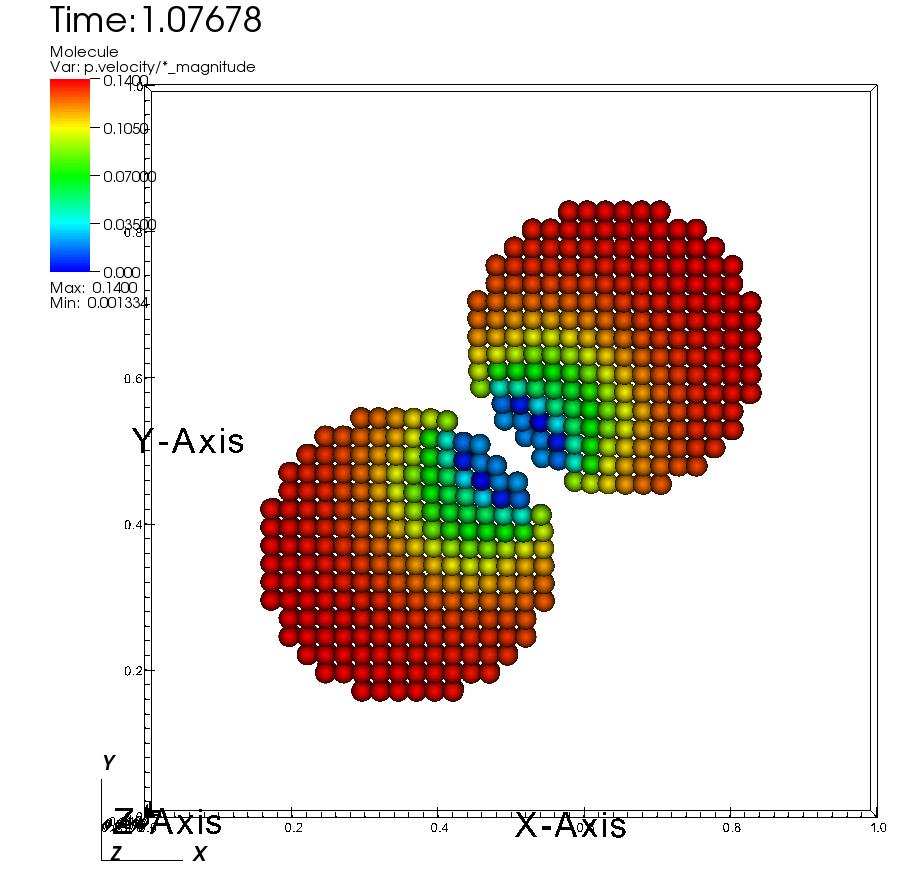
\includegraphics[scale=.25]{disks.png}
  \caption{Colliding elastic disks.  Particles colored according to
velocity magnitude.}
  \label{figdisks}
\end{figure}

Additional data is available within the uda in the form of "dat" files.
In this case, both the kinetic and strain energies are avaiable and can
be plotted to create a graph similar to that in Fig. 5a of \cite{sulskycmame}.
e.g. using gnuplot:

\begin{Verbatim}[fontsize=\footnotesize]
cd disks.uda.000
gnuplot
gnuplot> plot "StrainEnergy.dat", "KineticEnergy.dat"
gnuplot> quit
\end{Verbatim}

\section*{\center Taylor Impact Test}
\subsection*{\underline{Problem Description}}
This is a simulation of an Taylor impact experiment calculation from 
\cite{Gust82} in a copper cylinder at 718 K that is fired at a
rigid anvil at 188 m/s.  The copper cylinder has a length of 30 mm and
a diameter of 6 mm.  The cylinder rebounds from the anvil after 100 $\mu$s.
 
\subsection*{\underline{Simulation Specifics}}
\begin{description} 
\item [Component used:] \hfill MPM
\item [Input file name:] \hfill taylorImpact.ups
\item [Command used to run input file:]\hfill sus taylorImpact.ups
\item [Simulation Domain:]\hfill 8 mm x 33 mm x 8 mm

\item [Cell Spacing:]\hfill \\ 
  1/3 mm x 1/3 mm x 1/3 mm (Level 0)

\item [Example Runtimes:] \hfill \\
  1 hour   (1 processor, Xeon 3.16 GHz)\\

\item [Physical time simulated:] \hfill 100 $\mu$seconds

\item [Associate VisIt session:] \hfill taylorImpact.session

\end{description}

\section*{\underline{Results}}
Figure~\ref{fig:taylorImpact_slide} shows a snapshot from the end of the simulation.
There, the cylinder is allowed to slide laterally across the plate due
to the following optional specification in the \tt <contact> \normalfont
section:

\begin{Verbatim}[fontsize=\footnotesize]
        <direction>[1,1,1]</direction>
\end{Verbatim}

\begin{figure}
  \center
  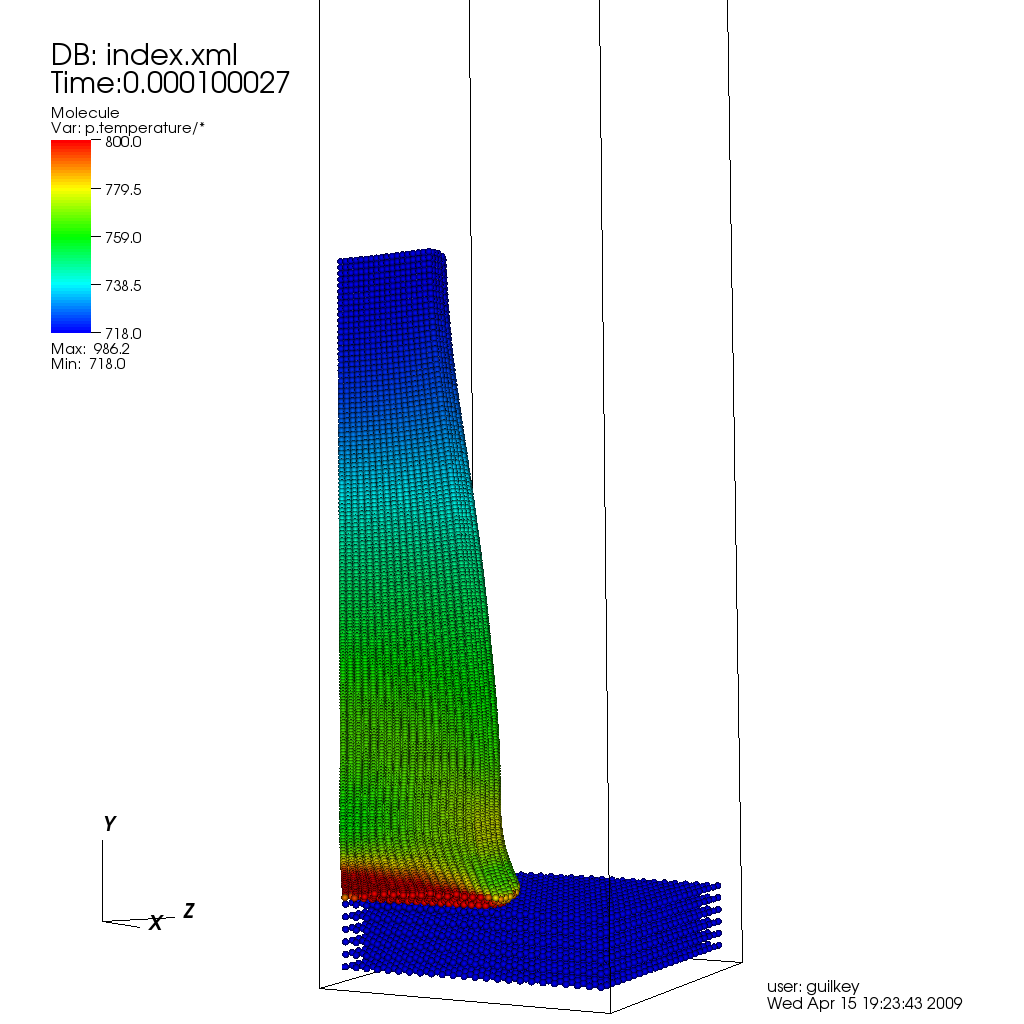
\includegraphics[scale=.25]{taylorImpact_slide.png}
  \caption{Taylor impact simulation with sliding between cylinder and
           target.  Particles colored according to temperature.}
  \label{fig:taylorImpact_slide}
\end{figure}

Figure~\ref{fig:taylorImpact_stick} shows a snapshot from the end of a
similar simulation.  In this case, the cylinder is restricted from sliding
laterally across the plate by altering the \tt <contact> \normalfont
section as follows:
\begin{Verbatim}[fontsize=\footnotesize]
        <direction>[0,1,0]</direction>
\end{Verbatim}

\begin{figure}
  \center
  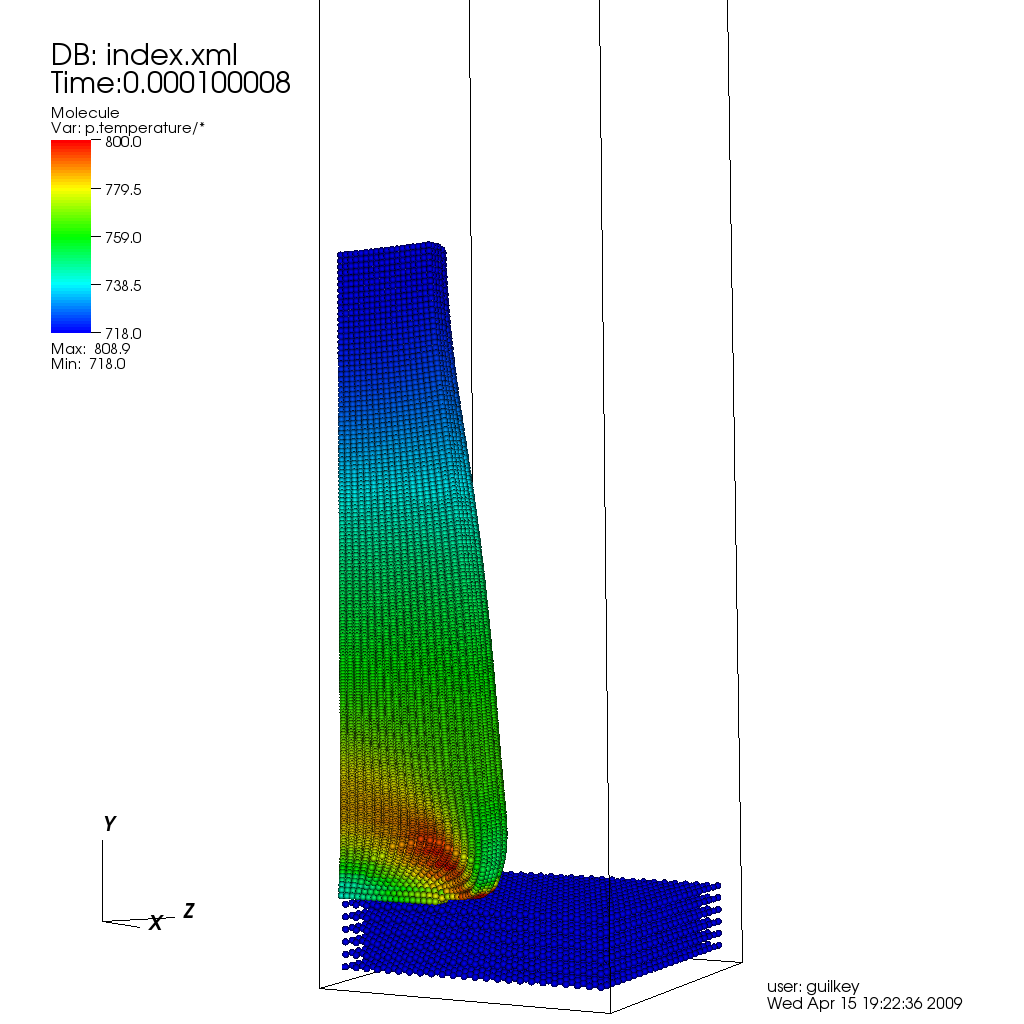
\includegraphics[scale=.25]{taylorImpact_stick.png}
  \caption{Taylor impact simulation with sliding prohibited between
           cylinder and target.  Particles colored according to temperature.}
  \label{fig:taylorImpact_stick}
\end{figure}


\section*{\center Sphere Rolling Down an Inclined Plane}
\subsection*{\underline{Problem Description}}
Here, a sphere of soft plastic, initially at rest, rolls under the
influence of gravity down a plane of a harder plastic.  Gravity is
oriented such that the plane is effectively angled at 45 degrees to
the horizontal.  This simulation demonstrates the effectiveness of
the contact algorithm, described in~\cite{bard01}.  Frictional
contact, using a friction coefficient of $\mu = 0.495$ causes the ball
to start rolling as it impacts the plane, after being dropped from
barely above it.  The same simulation is also run using a friction
coefficient of $\mu = 0.0$.  The difference in the results is shown
below.
 
\subsection*{\underline{Simulation Specifics}}
\begin{description} 
\item [Component used:] \hfill MPM
\item [Input file name:] \hfill inclinedPlaneSphere.ups
\item [Command used to run input file:]\hfill sus inclinedPlaneSphere.ups
\item [Simulation Domain:]\hfill    12.0 x 2.0 x 4.8 m

\item [Cell Spacing:]\hfill \\ 
.2 x .2 x .2 m (Level 0)

\item [Example Runtimes:] \hfill \\
 2.7 hours  (1 core, 3.16 GHz Xeon)\\

\item [Physical time simulated:] \hfill 2.2 seconds

\item [Associate VisIt session:] \hfill incplane.session

\end{description}

\section*{\underline{Results}}

Figure~\ref{figincplaneSphere_bigmu} and Figure~\ref{figincplaneSphere_0mu}
show snapshots of the simulation, as
the sphere is about halfway down the plane.
\begin{figure}
  \center
  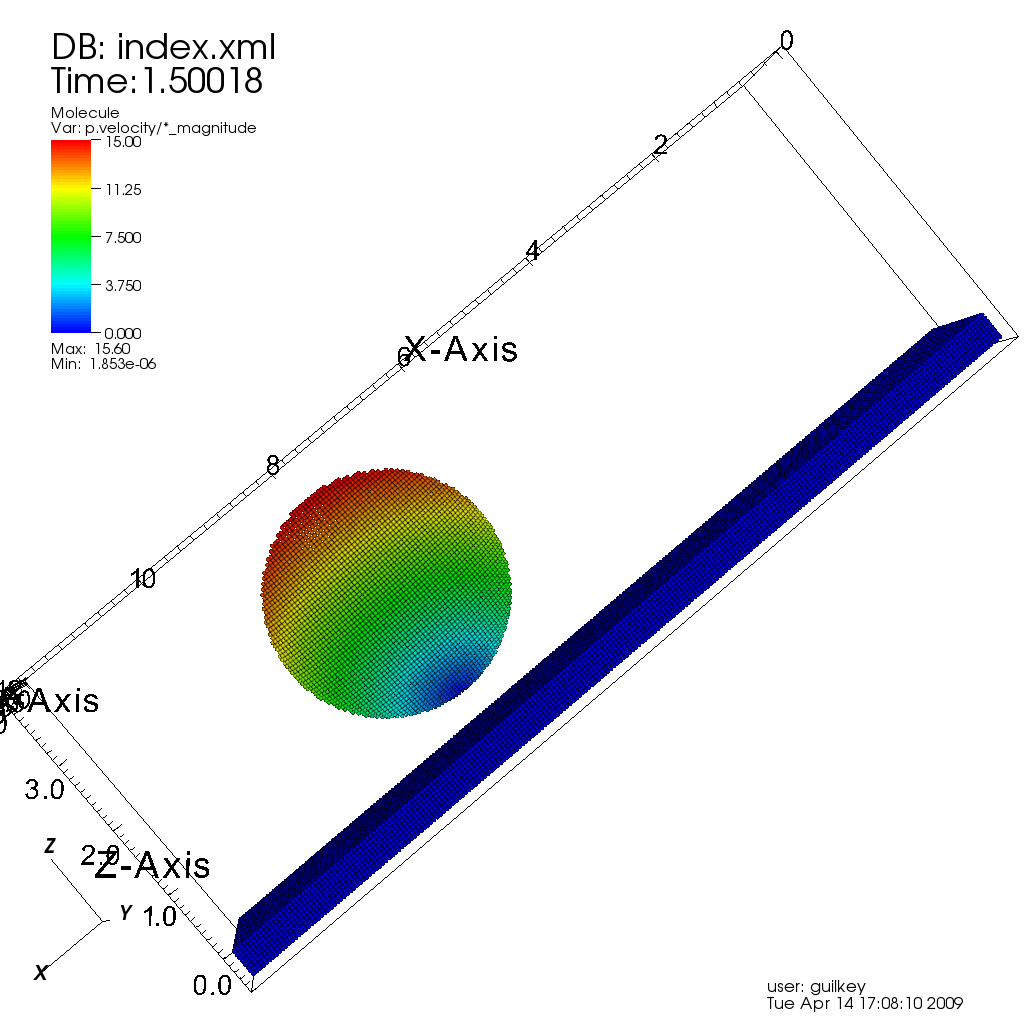
\includegraphics[scale=.25]{incplane_mu_495.png}
  \caption{Sphere rolling down an ``inclined" plane.  The gravity vector
is oriented at a 45 degree angle relative to the plane.  Particles are colored
by velocity magnitude. A friction coefficient of $\mu = 0.495$ is used.
Particles are colored according
to velocity magnitude, note that the particles at the top of the sphere
are moving most rapidly, and those near the surface of the plane are 
basically stationary, as expected.}
  \label{figincplaneSphere_bigmu}
\end{figure}

\begin{figure}
  \center
  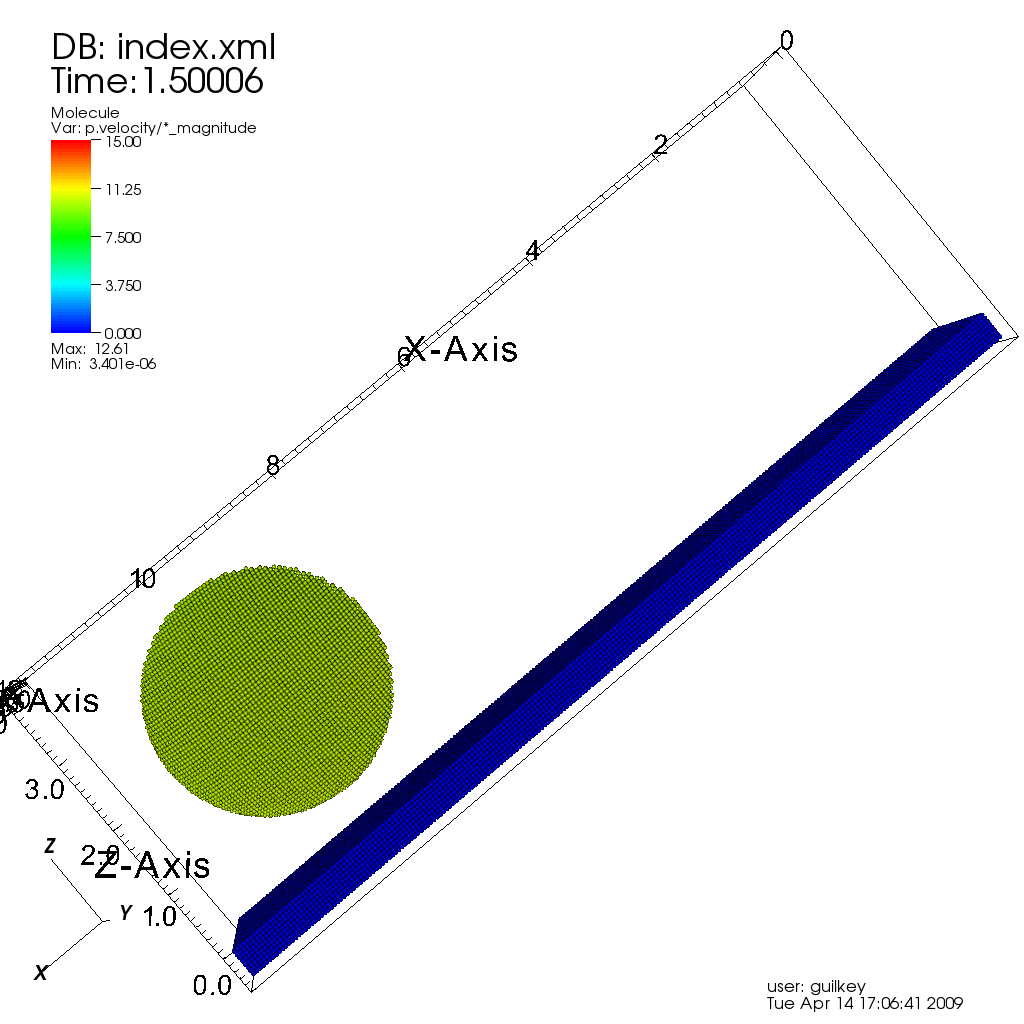
\includegraphics[scale=.25]{incplane_mu_0.png}
  \caption{Sphere rolling down an ``inclined" plane.  The gravity vector
is oriented at a 45 degree angle relative to the plane.  Particles are colored
by velocity magnitude.  A friction coefficient of $\mu = 0.0$ is used.
Particles are colored according to velocity magnitude.  In this case,
the particles throughout the sphere are moving at roughly the same velocity,
because the sphere is sliding as it moves down the plane, as opposed to
sticking and rolling.}
  \label{figincplaneSphere_0mu}
\end{figure}

\section*{\center Crushing a Foam Microstructure}
\subsection*{\underline{Problem Description}}
This calculation demonstrates two important strength of MPM.  The first
is the ability to quickly generate a computational representation of
complex geometries.  The second is the ability of the method to handle
large deformations, including self contact.

In particular, in this calculation a small sample of foam, the geometry
for which was collected using microCT, is represented via material points.
The sample is crushed to 87.5\% compaction through the use of a rigid plate, which
acts as a constant velocity boundary condition on the top of the sample.  This
calculation is a small example of those described in \cite{brydonfoam}.  The
geometry of the foam is created by image procesing the CT data, and based
on the intensity of each voxel in the image data, the space represented
by that voxel either recieves a particle with the material properties of the
foam's constituent material, or is left as void space.  This particle
representation avoids the time consuming steps required to build a suitable
unstructured mesh for this very complicated geometry.
 
\subsection*{\underline{Simulation Specifics}}
\begin{description} 
\item [Component used:] \hfill MPM
\item [Input file name:] \hfill foam.ups
\item [Instruction to run input file:]

First, copy foam.ups and foam.pts.gz to the same directory as sus.
Adjust the number of patches in the ups file based on
the number of processors available to you for this run.
First, uncompress the pts file:
\begin{Verbatim}[fontsize=\footnotesize]
 gunzip foam.pts.gz
\end{Verbatim}

Then the command:
\begin{Verbatim}[fontsize=\footnotesize]
 tools/pfs/pfs foam.ups
\end{Verbatim}
will divide the foam.pts
file, which contains the geometric description of the foam,
into number of patches smaller files, named foam.pts.0,
foam.pts.1, etc.  This is done so that for large simulations,
each processor is only reading that data which it needs, and
prevents the thrashing of the file system that would occur
if each processor needed to read the entire pts file.  This
command only needs to be done once, or anytime the patch
distibution is changed.  Note that this step must be done even
if only one processor is available.

To run this simulation:
\begin{Verbatim}[fontsize=\footnotesize]
  mpirun -np NP sus foam.ups
\end{Verbatim}
where NP is the number of processors being used.

\item [Simulation Domain:]\hfill  0.2 X 0.2 X 0.2125 mm

\item [Number of Computational Cells:]\hfill \\ 
102 X 102 X 85 (Level 0)

\item [Example Runtimes:] \hfill \\
2.4 hours  (4 cores, 3.16 GHz Xeon)\\

\item [Physical time simulated:] \hfill 3.75 seconds

\item [Associated VisIt session 1:] \hfill foam.iso.session
\item [Associated VisIt session 2:] \hfill foam.part.session

\end{description}

\section*{\underline{Results}}

Figure~\ref{figfoam} shows a snapshot of the simulation via isosurfacing,
as the foam is at about 50\% compaction.
\begin{figure}
  \center
  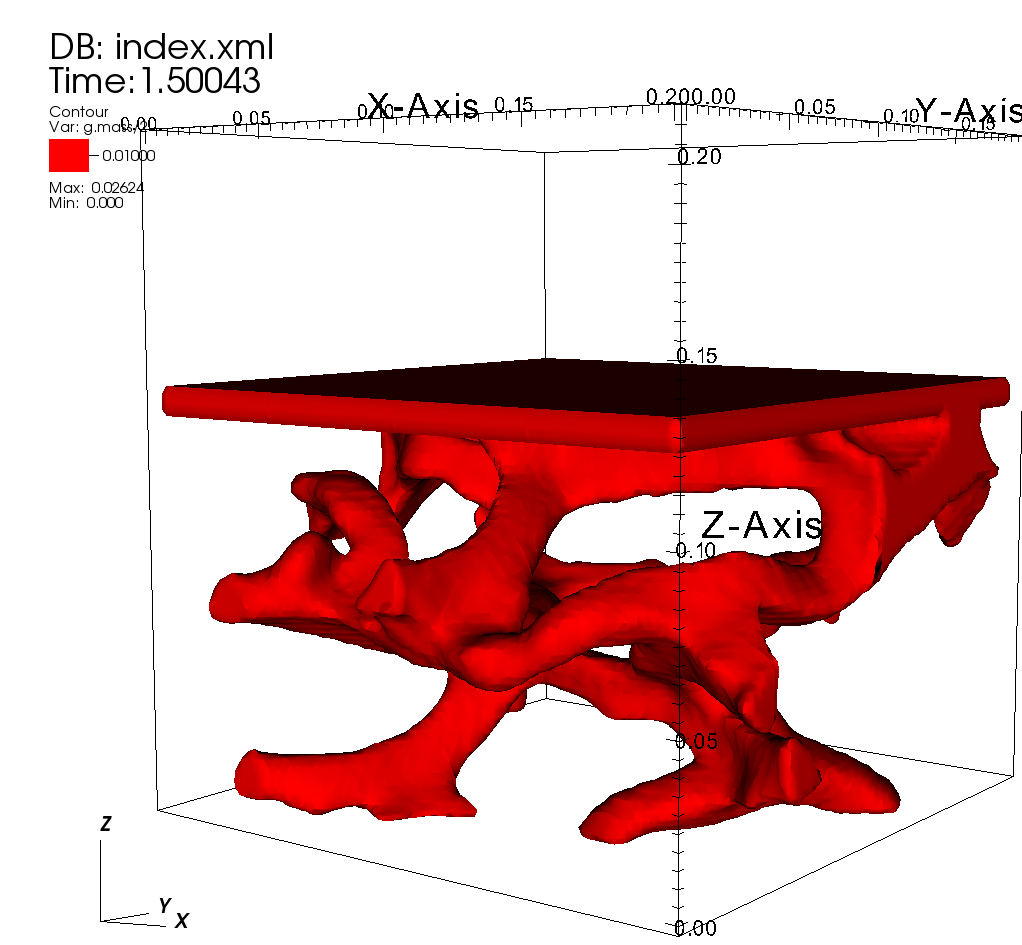
\includegraphics[scale=.15]{foam_iso.png}
  \caption{Compaction of a foam microstructure shown via isosurfacing.}
  \label{figfoam}
\end{figure}

Figure~\ref{figfoampart} shows a snapshot of the simulation via particles
colored by equivalent stress as the foam is at about 60\% compaction.
\begin{figure}
  \center
  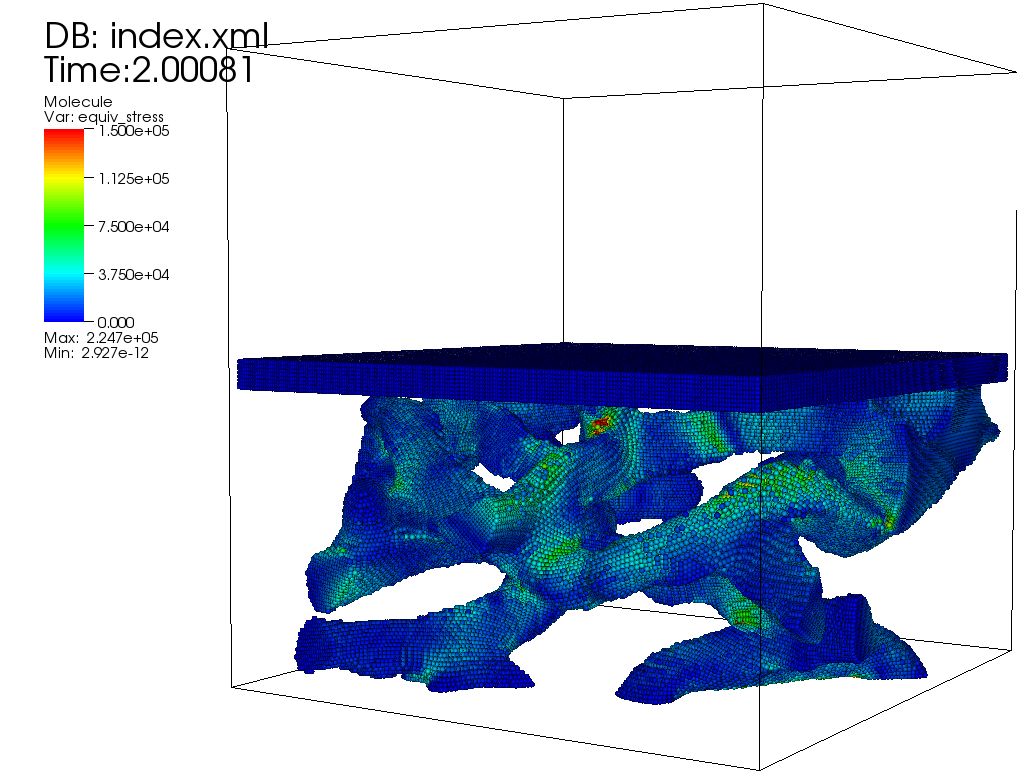
\includegraphics[scale=.15]{foam_part.png}
  \caption{Compaction of a foam microstructure rendered as particles colored
           by equivalent stress.}
  \label{figfoampart}
\end{figure}

In this simulation, the reaction forces at 5 of the 6 computational boundaries
are also recorded and can be viewed using a simple plotting package such
as gnuplot.  At each timestep, the internal force at each of the boundaries
is accumulated and stored in ``dat" files within the uda,
e.g. BndyForce\_zminus.dat.  Because the reaction force is a vector, it
is enclosed in square brackets which may be removed by use of a script in
the inputs directory:

\begin{Verbatim}[fontsize=\footnotesize]
cd foam.uda.000
../inputs/ICE/Scripts/removeBraces BndyForce\_zminus.dat
gnuplot
gnuplot> plot "BndyForce\_zminus.dat" using 1:4
gnuplot> quit
\end{Verbatim}

These reaction forces are similar to what would be measured on a mechanical
testing device, and help to understand the material behavior.

\section*{\center Hole in an Elastic Plate}
\subsection*{\underline{Problem Description}}
A flat plate with a hole in the center is loaded in tension.  To achieve a
quasi-static solution, the load is applied slowly and a viscous damping force
is used to reduce transients in the solution.  As such, this simulation
demonstrates those two capabilities.  Specifically, take note of:
\begin{Verbatim}[fontsize=\footnotesize]
       <use_load_curves> true </use_load_curves>
       <artificial_damping_coeff>1.0</artificial_damping_coeff>
\end{Verbatim}
in the \tt <MPM> \normalfont section of the input file, and:
\begin{Verbatim}[fontsize=\footnotesize]
   <PhysicalBC>
     <MPM>
       <pressure>
	.
	.
	.
\end{Verbatim}
section below that.

 
\subsection*{\underline{Simulation Specifics}}
\begin{description} 
\item [Component used:] \hfill MPM
\item [Input file name:] \hfill holePlate.ups
\item [Command used to run input file:]\hfill sus holePlate.ups
\item [Simulation Domain:]\hfill 5.0 m x 5.0 m x 0.1 m

\item [Cell Spacing:]\hfill \\ 
  0.1 m x 0.1 m x 0.1 m (Level 0)

\item [Example Runtimes:] \hfill \\
 2 minutes  (1 processor, Xeon 3.16 GHz)\\

\item [Physical time simulated:] \hfill 10 seconds

\item [Associate VisIt session:] \hfill holeInPlate.session

\end{description}

\section*{\underline{Results}}

Figure~\ref{fig:holeInPlate} shows a snapshot of the equivalent stress
throughout the plate, as well as the load applied to the vectors near the
edge of the plate.  Expected maximum stress is $300 Pa$.  The $238 Pa$ maximum
observed here is significantly lower, but upon doubling the resolution in the
x and y directions, the maximum stress is $308 Pa$.
\begin{figure}
  \center
  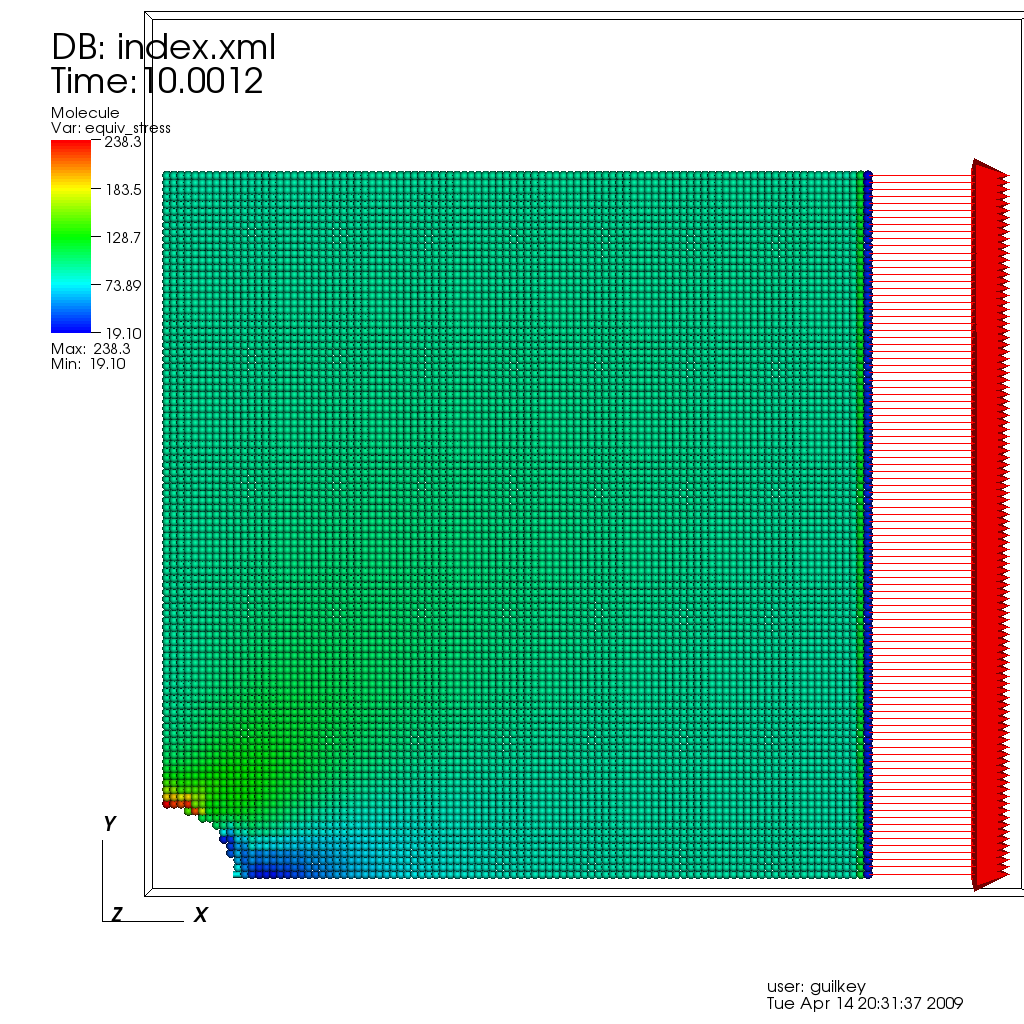
\includegraphics[scale=.25]{holeInPlate.png}
  \caption{Elastic plate with a hole loaded in tension.  Particles are
           colored by equivalent stress, vectors indicate applied load.}
  \label{fig:holeInPlate}
\end{figure}
\newpage

\section*{\center Tungsten Sphere Impacting a Steel Target}
\subsection*{\underline{Problem Description}}
A $1 mm$ tungsten sphere with an initial velocity of $5000 m/s$
impacts a steel target.  Axisymmetric conditions are used in this case,
conversion of the input file to the full 3D simulation is straightforward.
The user may wish to do both simulations of both to gain confidence in the
applicability of axisymmetry. 

This simulation exercises the \tt elastic\_plastic \normalfont
constitutive model for the
steel material. This includes sub-models for equations of state,
variable shear modulus, melting, plasticity, etc.  The tungsten is modeled
using the \tt comp\_neo\_hook\_plastic, \normalfont which is simple vonMises
plasticity with linear hardening.  One difficulty with using the more 
sophisticated models is that parameters can be difficult to find for many
materials.

\subsection*{\underline{Simulation Specifics}}
\begin{description}
\item [Component used:] \hfill MPM
\item [Input file name:] \hfill WSphereIntoSteel.axi.ups
\item [Command used to run input file:]\hfill sus WSphereIntoSteel.axi.ups
\item [Simulation Domain:]\hfill 1.0 cm x 1.5 cm x axisymmetric

\item [Cell Spacing:]\hfill \\
  0.333 mm x 0.333 mm x axisymmetry (Level 0)

\item [Example Runtimes:] \hfill \\
 15 seconds  (1 processor, Xeon 3.16 GHz)\\

\item [Physical time simulated:] \hfill 4 $\mu$seconds

\item [Associate VisIt session:] \hfill WSphereSteel.session

\end{description}

\section*{\underline{Results}}

Figure~\ref{fig:WSphereSteelInit} shows the initial configuration for
this simulation, with particles colored by the magnitude of their velocity.
Figure~\ref{fig:WSphereSteelFinal} shows the state of the simulation after
$4 \mu$seconds this simulation, with particles still colored by velocity
magnitude.

\begin{figure}
  \center
  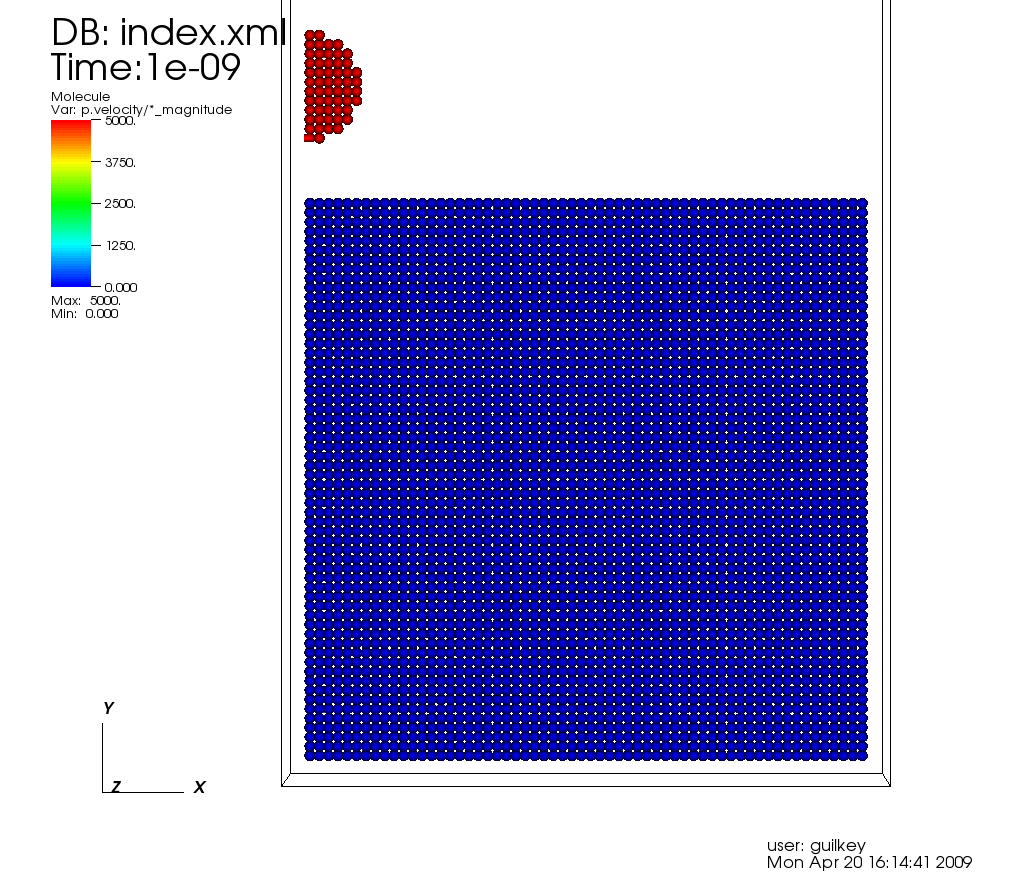
\includegraphics[scale=.25]{WShereInitAxi.png}
  \caption{Initial configuration of hypervelocity impact of tungsten sphere
           into a steel target.  Particles are
           colored by velocity magnitude.}
  \label{fig:WSphereSteelInit}
\end{figure}
\newpage
\begin{figure}
  \center
  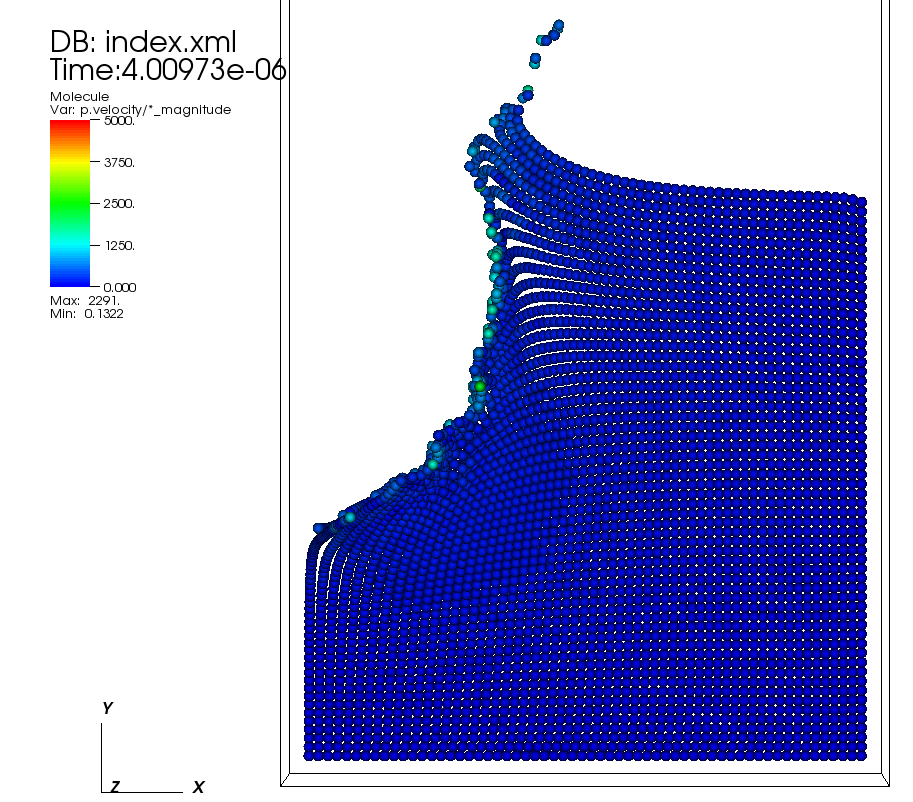
\includegraphics[scale=.25]{WShereFinalAxi.png}
  \caption{State of the tunsgsten and steel after $4 \mu$seconds.
           Particles are colored by velocity magnitude.}
  \label{fig:WSphereSteelFinal}
\end{figure}

\subsection{References}
\bibliographystyle{plain}
\bibliography{mpm}




